\باب{کمپیوٹر با}
  ارتقائی طور پر کمپیوٹر الف  ایک قدیم  مشین ہے جو  چند سادہ ہدایت پر عمل درآمد کر سکتا ہے۔ اس باب میں  ارتقا کی اگلی کڑی  پر غور کیا جائے گا جسے ہم کمپیوٹر با کہیں گے۔ کمپیوٹر با چھلانگ  کی ہدایات  جانتا ہے جو   برنامہ  کے کسی   حصے پر دوبارہ  عمل کرنے  یا اس حصے کو نظر انداز کرنے پر کمپیوٹر کو  مجبور کر سکتی ہیں۔ جیسا آپ جلد جان پائیں گے،چھلانگ  ہدایات  کی بدولت   کمپیوٹر کی طاقت بہت زیادہ  بڑھتی ہے۔
  
  \حصہ{دو طرفہ دفاتر}
  تاروں کی  برقی گنجائش کم کرنے کی غرض سے ہم کمپیوٹر با   کے ہر ایک دفتر اور \عددی{W} گزرگاہ کے بیچ   تاروں کا صرف ایک سلسلہ بچھائیں گے۔  شکل \حوالہ{شکل_کمپیوٹر_با_دو_طرفہ_دفتر}-الف   میں   اس تصور کی وضاحت کی گئی ہے۔ درآمدی اور برآمدی پنیے آپس میں جوڑے گئے ہیں؛ گزرگاہ  تک  تاروں کا  صرف  ایک گروہ  جاتا ہے۔
  
کیا درآمدی اور برآمدی پنیے آپس میں جوڑنا کوئی  مسئلہ کھڑا کرتا ہے؟ جی نہیں۔ کمپیوٹر کی دوڑ کے دوران کسی ایک وقت پر  \قول{  لاد } اور\قول{  مجاز } میں  سے  صرف ایک  فعال ہو گا۔ فعال \قول{لاد}  کی صورت میں  ثنائی مواد گزرگاہ سے دفتر  کی  درآمد    کی جانب گامزن ہو گا؛ لاد  عمل کے دوران ، برآمدی راہیں \اصطلاح{   غیر وابسطہ   }\فرہنگ{غیر وابسطہ}\حاشیہب{floating}\فرہنگ{floating}ہوں گی۔ اس کے برعکس،  فعال \قول{مجاز} کی صورت میں ،  ثنائی مواد دفتر سے  گزرگاہ کی طرف گامزن ہو گا، اور درآمدی راہیں غیر وابسطہ ہوں گی۔

\begin{figure}
\centering
\begin{subfigure}{1\textwidth}
\centering
\begin{tikzpicture}
\pgfmathsetmacro{\klshift}{0.25}
\pgfmathsetmacro{\knshift}{0.07}
\pgfmathsetmacro{\kmv}{0.15}
\pgfmathsetmacro{\knshift}{0.07}
\pgfmathsetmacro{\kpin}{0.50}
\pgfmathsetmacro{\kpina}{1}
\pgfmathsetmacro{\kpsep}{0.40}			%pin to pin distance
\pgfmathsetmacro{\kW}{\kpsep}
\pgfmathsetmacro{\kulV}{0.40}			%edge clearance along vertical edge
\pgfmathsetmacro{\kulH}{0.40}
\pgfmathsetmacro{\kdimX}{2*\kulH+3*\kpsep}
\pgfmathsetmacro{\kdimY}{2*\kulV+2*\kpsep}		%two spaces between 3 pins
\pgfmathsetmacro{\ksepX}{\kdimX+6*\kW}
\pgfmathsetmacro{\ksepY}{\kdimY+3*\kW}
\kBOX[uu0]{0}{0}{4}{3}{0.50}
\draw[thin](uu0-center)node[rectangle,inner sep=0pt,text width=2cm, align=center]{\small{\RTL{سہ حال\\ دفتر}}};
\foreach \n/\m/\q in {3/0/3,2/1/2,1/2/1,0/3/0}\draw[thin](uu0bpb\n)--++(0,-\kpin-\m*\kW/2)--++(\kulV+\kpsep+\m*\kpsep+\m*\kW/2,0)coordinate(uu0d\n)--++(0,\kdimY+2*\kpin+\m*\kW)coordinate(uu0u\n)-|(uu0dpb\q);
\draw[thin](uu0apb0)--++(-\kpin,0)node[left]{مجاز};
\draw[thin](uu0apb1)--++(-\kpin,0)node[left]{ساعت};
\draw[thin](uu0apb2)--++(-\kpin,0)node[left]{لاد};
\draw[thin](uu0apcu1)--(uu0apcm1)--(uu0apcd1);
\foreach \n/\m in {0/3,1/2,2/1,3/0}\draw[thin](\ksepX+\n*\kW,\ksepY)coordinate(w\m)--++(0,-4);
\draw($(w0)!0.5!(w3)$)node[above]{گزرگاہ};
\draw[thin]($(uu0d0)!0.5!(uu0u0)$)++(0,-1.5*\kW)coordinate(kA)--(kA-|w3);
\draw[thin]($(uu0d1)!0.5!(uu0u1)$)++(0,-0.5*\kW)coordinate(kA)--(kA-|w2);
\draw[thin]($(uu0d2)!0.5!(uu0u2)$)++(0,+0.5*\kW)coordinate(kA)--(kA-|w1);
\draw[thin]($(uu0d3)!0.5!(uu0u3)$)++(0,1.5*\kW)coordinate(kA)--(kA-|w0);
\end{tikzpicture}
\caption{}
\end{subfigure}
\begin{subfigure}{1\textwidth}
\centering
\begin{tikzpicture}
\pgfmathsetmacro{\klshift}{0.25}
\pgfmathsetmacro{\knshift}{0.07}
\pgfmathsetmacro{\kmv}{0.15}
\pgfmathsetmacro{\knshift}{0.07}
\pgfmathsetmacro{\kpin}{0.50}
\pgfmathsetmacro{\kpina}{1}
\pgfmathsetmacro{\kpsep}{0.40}			%pin to pin distance
\pgfmathsetmacro{\kW}{\kpsep}
\pgfmathsetmacro{\kulV}{0.40}			%edge clearance along vertical edge
\pgfmathsetmacro{\kulH}{0.40}
\pgfmathsetmacro{\kdimX}{2*\kulH+3*\kpsep}
\pgfmathsetmacro{\kdimY}{2*\kulV+2*\kpsep}		%two spaces between 3 pins
\pgfmathsetmacro{\ksepX}{\kdimX+6*\kW}
\pgfmathsetmacro{\ksepY}{\kdimY+0*\kW}
\pgfmathsetmacro{\kpsepSmall}{\kdimY/4}
\kBOX[uu0]{0}{0}{4}{3}{0.50}
\draw[thin](uu0-center)node[rectangle,inner sep=0pt,text width=2cm, align=center]{\small{\RTL{سہ حال دفتر\\ دخول و خروج\\ اندرونی جڑا}}};
\draw[thin](uu0apb0)--++(-\kpin,0)node[left]{مجاز};
\draw[thin](uu0apb1)--++(-\kpin,0)node[left]{ساعت};
\draw[thin](uu0apb2)--++(-\kpin,0)node[left]{لاد};
\draw[thin](uu0apcu1)--(uu0apcm1)--(uu0apcd1);
\foreach \n/\m in {0/3,1/2,2/1,3/0}\draw[thin](\ksepX+\n*\kW,\ksepY)coordinate(w\m)--++(0,-\kdimY);
\draw($(w0)!0.5!(w3)$)node[above]{گزرگاہ};
\draw[thin](\kdimX,0.5*\kpsepSmall)coordinate(kA)--(kA-|w0);
\draw[thin](\kdimX,1.5*\kpsepSmall)coordinate(kA)--(kA-|w1);
\draw[thin](\kdimX,2.5*\kpsepSmall)coordinate(kA)--(kA-|w2);
\draw[thin](\kdimX,3.5*\kpsepSmall)coordinate(kA)--(kA-|w3);
\end{tikzpicture}
\caption{}
\end{subfigure}
\begin{subfigure}{1\textwidth}
\centering
\begin{tikzpicture}
\pgfmathsetmacro{\klshift}{0.25}
\pgfmathsetmacro{\knshift}{0.07}
\pgfmathsetmacro{\kmv}{0.15}
\pgfmathsetmacro{\knshift}{0.07}
\pgfmathsetmacro{\kpin}{0.50}
\pgfmathsetmacro{\kpina}{1}
\pgfmathsetmacro{\kpsep}{0.40}			%pin to pin distance
\pgfmathsetmacro{\kW}{\kpsep}
\pgfmathsetmacro{\kulV}{0.40}			%edge clearance along vertical edge
\pgfmathsetmacro{\kulH}{0.40}
\pgfmathsetmacro{\kdimX}{2*\kulH+3*\kpsep}
\pgfmathsetmacro{\kdimY}{2*\kulV+2*\kpsep}		%two spaces between 3 pins
\pgfmathsetmacro{\ksepX}{\kdimX+6*\kW}
\pgfmathsetmacro{\ksepY}{\kdimY+0*\kW}
\pgfmathsetmacro{\kpsepSmall}{\kdimY/4}
\kBOX[uu0]{0}{0}{4}{3}{0.50}
\draw[thin](uu0-center)node[rectangle,inner sep=0pt,text width=2cm, align=center]{\small{\RTL{دو طرفہ\\ دفتر}}};
\draw[thin](uu0apb0)--++(-\kpin,0)node[left]{$E$};
\draw[thin](uu0apb1)--++(-\kpin,0)node[left]{$CLK$};
\draw[thin](uu0apb2)--++(-\kpin,0)node[left]{$L$};
\draw[thin](uu0apcu1)--(uu0apcm1)--(uu0apcd1);
\draw[thick](\ksepX+\kW,\ksepY) rectangle ++(1*\kW,-\kdimY);
\draw[thick](\ksepX+1.5*\kW,\ksepY)node[above]{گزرگاہ};
\draw[thin](\kdimX,0.5*\kdimY)--++(\kW,\kW)coordinate[pos=0.5](aa);
\draw[thin](\kdimX,0.5*\kdimY)--++(\kW,-\kW)coordinate[pos=0.5](bb);
\draw[thin](\ksepX+\kW,0.5*\kdimY)--++(-\kW,\kW)coordinate[pos=0.5](cc);
\draw[thin](\ksepX+\kW,0.5*\kdimY)--++(-\kW,-\kW)coordinate[pos=0.5](dd);
\draw[thin](aa)--(cc);
\draw[thin](bb)--(dd);
\end{tikzpicture}
\caption{}
\end{subfigure}
\caption{دو طرفہ دفتر}
\label{شکل_کمپیوٹر_با_دو_طرفہ_دفتر}
\end{figure}
سہ  حال دفتر کے درآمدی اور برآمدی پنیوں کو   مخلوط  دور ساز   اندرونی طور  پر  آپس میں جوڑ  سکتا ہے۔ اس سے نا صرف تاروں کی برقی گنجائش کم ہو گی بلکہ  درآمدی و برآمدی   پنیوں کی تعداد بھی کم ہو گی۔ مثلاً، شکل \حوالہ{شکل_کمپیوٹر_با_دو_طرفہ_دفتر}-ب  میں آٹھ کی بجائے چار درآمدی و برآمدی پنیے ہیں۔ 

شکل \حوالہ{شکل_کمپیوٹر_با_دو_طرفہ_دفتر}-ج  میں سہ حال دفتر ، جس کے درآمدی اور برآمدی  راہ  اندرونی طور پر   آپس میں جڑے ہیں، کی علامت  پیش ہے۔ دو طرفہ تیر ہمیں یاد دلاتا ہے کہ یہ راہ\اصطلاح{ دو طرفہ }\فرہنگ{دو طرفہ}\حاشیہب{bidirectional}\فرہنگ{bidirectional} ہے؛  اس پر  مواد  کسی بھی  طرف  چل سکتا ہے۔

\حصہ{طرز تعمیر}
شکل \حوالہ{شکل_کمپیوٹر_با_تعمیر}  میں کمپیوٹر با کی طرز تعمیر پیش ہے۔   دفاتر کے وہ برآمدات جو  گزرگاہ \عددی{W} سے منسلک   ہیں سہ حال ہیں؛ جو \عددی{W} گزرگاہ سے منسلک نہیں، وہ دو حال ہیں۔ یہاں بھی ہر ایک دفتر کو  قابو و ترتیب کار قابو اشارات (جو یہاں دکھائے نہیں گئے)  بھیجتا ہے۔  قابو اشارات ساعت کے   اگلے کنارہ چڑھائی پر دفتر کو لادنے،  یا مجاز  ہونے، یا کسی دوسرے مقصد کے لئے تیار کرتے ہیں۔ ہر ڈبے کی مختصر تفصیل درج ذیل ہے۔

\begin{figure}
\centering
\begin{tikzpicture}
\pgfmathsetmacro{\klshift}{0.25}
\pgfmathsetmacro{\knshift}{0.07}
\pgfmathsetmacro{\kmv}{0.15}
\pgfmathsetmacro{\knshift}{0.07}
\pgfmathsetmacro{\kpin}{0.50}
\pgfmathsetmacro{\kpina}{1}
\pgfmathsetmacro{\kpsep}{0.40}			%pin to pin distance
\pgfmathsetmacro{\kW}{0.5}
\pgfmathsetmacro{\kAr}{0.35}
\pgfmathsetmacro{\kulV}{0.40}			%edge clearance along vertical edge
\pgfmathsetmacro{\kulH}{0.40}
\pgfmathsetmacro{\kdimX}{2.5}
\pgfmathsetmacro{\kdimXA}{2.0}
\pgfmathsetmacro{\kdimY}{1.5}		%two spaces between 3 pins
\pgfmathsetmacro{\ksepXW}{1}
\pgfmathsetmacro{\ksepX}{\kdimX+2*\ksepXW+\kW}
\pgfmathsetmacro{\ksepYA}{2}
\pgfmathsetmacro{\ksepYB}{2.5}
%
%W bus
\draw[thick](\kdimX+\ksepXW,\kdimY) rectangle ++(\kW,-8*\ksepYA);
\draw[](\kdimX+\ksepXW+0.5*\kW,\kdimY)node[yshift=3ex,rectangle,inner sep=0pt, text width=2cm,align=center]{\RTL{$W$ گزرگاہ}} node[below]{$16$};

%kLa, kRa  points to lower left and upper right corners
\draw(0,0)coordinate(kAnchor)coordinate(kLa)  [thick] rectangle ++(\kdimX,\kdimY)coordinate(kRa) node[pos=0.5,rectangle,inner sep=0pt,text width=2.75cm,align=center]{\RTL{مرموز کار برائے\\ سادس عشری\\ ٹائپ کار تختی}};
\draw[thick,latex-](kAnchor)++(0,0.75*\kdimY)--++(-\kpin,0)node[left]{\RTL{تشکر}};
\draw[thick](kAnchor)++(0,0.25*\kdimY)--++(-1.5*\kpin,0)coordinate(readyOut);
%kLb, kRb  points to lower left and upper right corners
\draw(kAnchor)++(0,-1*\ksepYA)coordinate(kAnchor)coordinate(kRb)  [thick] rectangle ++(\kdimX,\kdimY)coordinate(kRb) node[pos=0.5,rectangle,inner sep=0pt,text width=2.75cm,align=center]{\RTL{داخلی روزن\\ 1}};
%arrow head vertical
\draw[thick](kAnchor)++(0.5*\kdimX,\kdimY)coordinate(kA)node[above]{$8$}--++(-\kAr,\kAr)coordinate[pos=0.5](aa)  (kA)--++(\kAr,\kAr)coordinate[pos=0.5](bb)  (aa)--(aa|-kLa)  (bb)--(bb|-kLa);
%arrow head horizontal
\draw[thick](kAnchor)++(\kdimX+\ksepXW,0.5*\kdimY)coordinate(kA)--++(-\kAr,\kAr)coordinate[pos=0.5](aa)  (kA)--++(-\kAr,-\kAr)coordinate[pos=0.5](bb)  (aa)--(aa-| kRb)  (bb)--(bb-|kRb)  (kA)++(-0.5*\ksepXW,0)node[]{$8$};
%kLc, kRc  points to lower left and upper right corners
\draw(kAnchor)++(0,-1*\ksepYA)coordinate(kAnchor)  [thick] rectangle ++(\kdimX,\kdimY)
 node[pos=0.5,rectangle,inner sep=0pt,text width=2.75cm,align=center]{\RTL{داخلی روزن\\ 2}};
 \draw[thick,latex-](kAnchor)++(0,0.75*\kdimY)node[above left]{$0$}--++(-1.5*\kpin,0)node[left]{\RTL{تیار}}--(readyOut);
  \draw[thick,latex-](kAnchor)++(0,0.25*\kdimY)node[above left]{$7$}--++(-1*\kpin,0)node[left,yshift=-1ex,rectangle,text width=1.25cm,align=center]{\RTL{سلسلہ وار\\ درآمد}};
%arrow head horizontal
\draw[thick](kAnchor)++(\kdimX+\ksepXW,0.5*\kdimY)coordinate(kA)--++(-\kAr,\kAr)coordinate[pos=0.5](aa)  (kA)--++(-\kAr,-\kAr)coordinate[pos=0.5](bb)  (aa)--(aa-| kRb)  (bb)--(bb-|kRb)  (kA)++(-0.5*\ksepXW,0)node[]{$8$};
%kLd, kRd  points to lower left and upper right corners
\draw(kAnchor)++(0,-1*\ksepYA)coordinate(kAnchor)   [thick] rectangle ++(\kdimX,\kdimY) 
node[pos=0.5,rectangle,inner sep=0pt,text width=2.75cm,align=center]{\RTL{برنامہ \\گنت کار}};
%bidirectional arrow head horizontal
\draw[thick](kAnchor)++(\kdimX+\ksepXW,0.5*\kdimY)coordinate(kA)--++(-\kAr,\kAr)coordinate[pos=0.5](aa)  (kA)--++(-\kAr,-\kAr)coordinate[pos=0.5](bb)  (kAnchor)++(\kdimX,0.5*\kdimY)coordinate(kA)--++(\kAr,\kAr)coordinate[pos=0.5](cc)  (kA)--++(\kAr,-\kAr)coordinate[pos=0.5](dd)  (aa)--(cc)  (bb)--(dd)  (kA)++(0.5*\ksepXW,0)node[]{$16$};

\draw(kAnchor)++(0,-1*\ksepYA)coordinate(kAnchor)   [thick] rectangle ++(\kdimX,\kdimY)
 node[pos=0.5,rectangle,inner sep=0pt,text width=2.75cm,align=center]{\RTL{دفتر پتہ}};
 %arrow head horizontal
\draw[thick](kAnchor)coordinate(kL)++(\kdimX+\ksepXW,0.5*\kdimY)coordinate(kA)++(0,0.5*\kAr)coordinate(aa) 
 (kA)++(0,-0.5*\kAr)coordinate(bb)  (kAnchor)++(\kdimX,0.5*\kdimY)coordinate(kA)--++(\kAr,\kAr)coordinate[pos=0.5](cc)  (kA)--++(\kAr,-\kAr)coordinate[pos=0.5](dd)  (aa)--(cc)  (bb)--(dd)  (kA)++(0.5*\ksepXW,0)node[]{$16$};
 
 \draw(kAnchor)++(0,-1*\ksepYA)coordinate(kAnchor)   [thick] rectangle ++(\kdimX,\kdimY)
 node[pos=0.5,rectangle,inner sep=0pt,text width=2.75cm,align=center]{64\,K \\ \RTL{حافظہ}};
 %arrow head vertical
\draw[thick](kAnchor)++(0.5*\kdimX,\kdimY)coordinate(kA)node[above,yshift=0.5ex]{$16$}--++(-\kAr,\kAr)coordinate[pos=0.65](aa)  (kA)--++(\kAr,\kAr)coordinate[pos=0.65](bb)  (aa)--(aa|-kL)  (bb)--(bb|-kL);
\draw[thick](kAnchor)++(0.5*\kdimX,0)coordinate(kA)coordinate(kB)--++(-\kAr,-\kAr)coordinate[pos=0.65](aa)  (kA)--++(\kAr,-\kAr)coordinate[pos=0.65](bb);

 \draw(kAnchor)++(0,-\ksepYB)coordinate(kAnchor)   [thick] rectangle ++(\kdimX,\kdimY)
 node[pos=0.5,rectangle,inner sep=0pt,text width=2.75cm,align=center]{\RTL{مواد دفتر}};
 \draw[thick](kAnchor)++(0.5*\kdimX,\kdimY)coordinate(kA)--++(-\kAr,\kAr)coordinate[pos=0.65](cc)  
 (kA)--++(\kAr,\kAr)coordinate[pos=0.65](dd)   (aa)--(cc)  (bb)--(dd);
 \draw[thick]($(kA)!0.5!(kB)$)node[]{$8$};
 
 %bidirectional arrow head horizontal
\draw[thick](kAnchor)++(\kdimX+\ksepXW,0.5*\kdimY)coordinate(kA)--++(-\kAr,\kAr)coordinate[pos=0.5](aa)  (kA)--++(-\kAr,-\kAr)coordinate[pos=0.5](bb)  (kAnchor)++(\kdimX,0.5*\kdimY)coordinate(kA)--++(\kAr,\kAr)coordinate[pos=0.5](cc)  (kA)--++(\kAr,-\kAr)coordinate[pos=0.5](dd)  (aa)--(cc)  (bb)--(dd)  (kA)++(0.5*\ksepXW,0)node[]{$8$};

 \draw(kAnchor)++(0,-\ksepYA)coordinate(kAnchor)   [thick] rectangle ++(\kdimX,\kdimY)
 node[pos=0.5,rectangle,inner sep=0pt,text width=2.75cm,align=center]{\RTL{دفتر ہدایت}};
  %arrow head horizontal
\draw[thick](kAnchor)coordinate(kL)++(\kdimX+\ksepXW,0.5*\kdimY)coordinate(kA)++(0,0.5*\kAr)coordinate(aa) 
 (kA)++(0,-0.5*\kAr)coordinate(bb)  (kAnchor)++(\kdimX,0.5*\kdimY)coordinate(kA)--++(\kAr,\kAr)coordinate[pos=0.5](cc)  (kA)--++(\kAr,-\kAr)coordinate[pos=0.5](dd)  (aa)--(cc)  (bb)--(dd)  (kA)++(0.5*\ksepXW,0)node[]{$8$};
\draw[thick](kAnchor)++(0.5*\kdimX,0)coordinate(kA)node[below]{$8$}++(-0.5*\kAr,0)coordinate(aa)  (kA)++(0.5*\kAr,0)coordinate(bb);
 
 \draw(kAnchor)++(0,-\ksepYA)coordinate(kAnchor)   [thick] rectangle ++(\kdimX,\kdimY)
 node[pos=0.5,rectangle,inner sep=0pt,text width=2.75cm,align=center]{\RTL{قابو و ترتیب کار}};
 \draw[thick](kAnchor)++(0.5*\kdimX,\kdimY)coordinate(kA)--++(-\kAr,\kAr)coordinate[pos=0.5](cc)  (kA)--++(\kAr,\kAr)coordinate[pos=0.5](dd)   (aa)--(cc)  (bb)--(dd); 
 
 \draw[thick](kAnchor)++(0.5*\kdimX,0)coordinate(kA)++(-0.5*\kAr,0)coordinate(aa)  (kA)++(0.5*\kAr,0)coordinate(bb)
 (kA)++(0,-\ksepYA+\kdimY)coordinate(kB)--++(-\kAr,\kAr)coordinate[pos=0.5](cc)  (kB)--++(\kAr,\kAr)coordinate[pos=0.5](dd)   (aa)--(cc)  (bb)--(dd)  (kB)node[below]{\RL{قابو لفظ}}; 
 
 \draw(\ksepX,-1*\ksepYA)coordinate(kAnchor)coordinate(kRb)  [thick] rectangle ++(\kdimXA,\kdimY)coordinate(kRb) node[pos=0.5,rectangle,inner sep=0pt,text width=2.75cm,align=center]{\RTL{دفتر \دفترالف}};
  %bidirectional arrow head horizontal
\draw[thick](kAnchor)++(-\ksepXW,0.5*\kdimY)coordinate(kA)--++(\kAr,\kAr)coordinate[pos=0.5](aa)  (kA)--++(\kAr,-\kAr)coordinate[pos=0.5](bb)  (kAnchor)++(0,0.5*\kdimY)coordinate(kA)--++(-\kAr,\kAr)coordinate[pos=0.5](cc)  (kA)--++(-\kAr,-\kAr)coordinate[pos=0.5](dd)  (aa)--(cc)  (bb)--(dd)  (kA)++(-0.5*\ksepXW,0)node[]{$8$};
 \draw[thick](kAnchor)++(0.5*\kdimXA,0)coordinate(kA)coordinate(kB)++(-0.5*\kAr,0)coordinate(aa)  
 (kA)++(0.5*\kAr,0)coordinate(bb);
 
  
 \draw(kAnchor)++(0,-\ksepYA)coordinate(kAnchor)coordinate(kAnchorB)   [thick] rectangle ++(\kdimXA,\kdimY)
 node[pos=0.5,rectangle,inner sep=0pt,text width=2.75cm,align=center]{\RTL{مرکز حساب و منطق}};
 
\draw[thick](kAnchor)++(0.5*\kdimXA,\kdimY)coordinate(kA)--++(-\kAr,\kAr)coordinate[pos=0.5](cc)  
 (kA)--++(\kAr,\kAr)coordinate[pos=0.5](dd)   (aa)--(cc)  (bb)--(dd)   ($(kA)!0.5!(kB)$)node[]{$8$};
  
  \draw[thick](kAnchor)++(-\ksepXW,0.5*\kdimY)coordinate(kA)--++(\kAr,\kAr)coordinate[pos=0.5](aa)  
   (kA)--++(\kAr,-\kAr)coordinate[pos=0.5](bb)  
   (kAnchor)++(0,0.5*\kdimY)coordinate(kA)++(0,0.5*\kAr)coordinate(cc)  (kA)++(0,-0.5*\kAr)coordinate(dd)
   (aa)--(cc)  (bb)--(dd)  ($(aa)!0.5!(dd)$)node[]{$8$}; 
 
\draw[thick](kAnchor)++(\kdimXA,0.5*\kdimY)coordinate(kA)++(0,0.5*\kAr)coordinate(aa)  
   (kA)++(0,-0.5*\kAr)coordinate(bb);
 
  \draw(kAnchor)++(\kdimXA+\ksepXW,0)coordinate(kAnchor)   [thick] rectangle ++(0.5*\kdimX,\kdimY)
 node[pos=0.5,rectangle,inner sep=0pt,text width=2.75cm,align=center]{\RTL{جھنڈے}};
 \draw[thick](kAnchor)++(0,0.5*\kdimY)coordinate(kA)--++(-\kAr,\kAr)coordinate[pos=0.5](cc)  
   (kA)--++(-\kAr,-\kAr)coordinate[pos=0.5](dd)  (aa)--(cc)  (bb)--(dd)  ($(aa)!0.5!(dd)$)node[]{$2$}; 
   
 \draw(kAnchorB)++(0,-\ksepYA)coordinate(kAnchor)   [thick] rectangle ++(\kdimXA,\kdimY)
 node[pos=0.5,rectangle,inner sep=0pt,text width=2.75cm,align=center]{\RTL{عارضی دفتر}};
 
   %bidirectional arrow head horizontal
\draw[thick](kAnchor)++(-\ksepXW,0.5*\kdimY)coordinate(kA)--++(\kAr,\kAr)coordinate[pos=0.5](aa)  (kA)--++(\kAr,-\kAr)coordinate[pos=0.5](bb)  (kAnchor)++(0,0.5*\kdimY)coordinate(kA)--++(-\kAr,\kAr)coordinate[pos=0.5](cc)  (kA)--++(-\kAr,-\kAr)coordinate[pos=0.5](dd)  (aa)--(cc)  (bb)--(dd)  (kA)++(-0.5*\ksepXW,0)node[]{$8$};
 \draw[thick](kAnchor)++(0.5*\kdimXA,0)coordinate(kA)coordinate(kB)++(-0.5*\kAr,0)coordinate(aa)  
 (kA)++(0.5*\kAr,0)coordinate(bb);
 
\draw[thick](kAnchor)++(0.5*\kdimXA,\kdimY)coordinate(kA)++(-0.5*\kAr,0)coordinate[](aa)  
 (kA)++(0.5*\kAr,0)coordinate[](bb);
\draw[thick](kAnchorB)++(0.5*\kdimXA,0)coordinate(kA)--++(-\kAr,-\kAr)coordinate[pos=0.5](cc)  
 (kA)--++(\kAr,-\kAr)coordinate[pos=0.5](dd)  (aa)--(cc)  (bb)--(dd)   ($(aa)!0.5!(dd)$)node[]{$8$};
 
\draw(kAnchor)++(0,-\ksepYA)coordinate(kAnchor)   [thick] rectangle ++(\kdimXA,\kdimY)
 node[pos=0.5,rectangle,inner sep=0pt,text width=2.75cm,align=center]{\RTL{دفتر \دفترب}};
 
   %bidirectional arrow head horizontal
\draw[thick](kAnchor)++(-\ksepXW,0.5*\kdimY)coordinate(kA)--++(\kAr,\kAr)coordinate[pos=0.5](aa)  (kA)--++(\kAr,-\kAr)coordinate[pos=0.5](bb)  (kAnchor)++(0,0.5*\kdimY)coordinate(kA)--++(-\kAr,\kAr)coordinate[pos=0.5](cc)  (kA)--++(-\kAr,-\kAr)coordinate[pos=0.5](dd)  (aa)--(cc)  (bb)--(dd)  (kA)++(-0.5*\ksepXW,0)node[]{$8$};
 \draw[thick](kAnchor)++(0.5*\kdimXA,0)coordinate(kA)coordinate(kB)++(-0.5*\kAr,0)coordinate(aa)  
 (kA)++(0.5*\kAr,0)coordinate(bb);
 
 \draw(kAnchor)++(0,-\ksepYA)coordinate(kAnchor)   [thick] rectangle ++(\kdimXA,\kdimY)
 node[pos=0.5,rectangle,inner sep=0pt,text width=2.75cm,align=center]{\RTL{دفتر \دفترج}};
 
   %bidirectional arrow head horizontal
\draw[thick](kAnchor)++(-\ksepXW,0.5*\kdimY)coordinate(kA)--++(\kAr,\kAr)coordinate[pos=0.5](aa)  (kA)--++(\kAr,-\kAr)coordinate[pos=0.5](bb)  (kAnchor)++(0,0.5*\kdimY)coordinate(kA)--++(-\kAr,\kAr)coordinate[pos=0.5](cc)  (kA)--++(-\kAr,-\kAr)coordinate[pos=0.5](dd)  (aa)--(cc)  (bb)--(dd)  (kA)++(-0.5*\ksepXW,0)node[]{$8$};
 \draw[thick](kAnchor)++(0.5*\kdimXA,0)coordinate(kA)coordinate(kB)++(-0.5*\kAr,0)coordinate(aa)  
 (kA)++(0.5*\kAr,0)coordinate(bb);
 
\draw(kAnchor)++(0,-\ksepYB)coordinate(kAnchor)coordinate(kAnchorC)   [thick] rectangle ++(\kdimXA,\kdimY)
 node[pos=0.5,rectangle,inner sep=0pt,text width=2.75cm,align=center]{\RTL{خارجی روزن 3}};
 
   %bidirectional arrow head horizontal
\draw[thick](kAnchor)++(-\ksepXW,0.5*\kdimY)coordinate(kA)++(0,0.5*\kAr)coordinate[](aa)
  (kA)++(0,-0.5*\kAr)coordinate[](bb)  (kAnchor)++(0,0.5*\kdimY)coordinate(kA)--++(-\kAr,\kAr)coordinate[pos=0.5](cc)  (kA)--++(-\kAr,-\kAr)coordinate[pos=0.5](dd)  (aa)--(cc)  (bb)--(dd)  (kA)++(-0.5*\ksepXW,0)node[]{$8$};
 \draw[thick](kAnchor)++(0.5*\kdimXA,0)coordinate(kA)coordinate(kB)++(-0.5*\kAr,0)coordinate(aa)  
 (kA)++(0.5*\kAr,0)coordinate(bb);

\draw(kAnchor)++(0,-\ksepYA)coordinate(kAnchor)   [thick] rectangle ++(\kdimXA,\kdimY)
 node[pos=0.5,rectangle,inner sep=0pt,text width=2.75cm,align=center]{\RTL{خارجی روزن 4}};
 \draw[thick,-latex](kAnchor)++(\kdimXA,0.25*\kdimY)node[above right]{$7$}--++(\ksepXW,0)node[right]{\RTL{تشکر}};
  \draw[thick,-latex](kAnchor)++(\kdimXA,0.75*\kdimY)node[above right]{$0$}--++(\ksepXW,0)node[right,rectangle,inner sep=0pt, text width=2cm]{\RTL{سلسلہ وار برآمد}};
   %bidirectional arrow head horizontal
\draw[thick](kAnchor)++(-\ksepXW,0.5*\kdimY)coordinate(kA)++(0,0.5*\kAr)coordinate[](aa)
  (kA)++(0,-0.5*\kAr)coordinate[](bb)  (kAnchor)++(0,0.5*\kdimY)coordinate(kA)--++(-\kAr,\kAr)coordinate[pos=0.5](cc)  (kA)--++(-\kAr,-\kAr)coordinate[pos=0.5](dd)  (aa)--(cc)  (bb)--(dd)  (kA)++(-0.5*\ksepXW,0)node[]{$8$};
 
 \draw(kAnchorC)++(\kdimXA+\ksepXW,0)coordinate(kAnchor)   [thick] rectangle ++(0.9*\kdimX,\kdimY)
 node[pos=0.5,rectangle,inner sep=0pt,text width=2.75cm,align=center]{\RTL{سادس عشری\\ نمائشی تختی}};
 
   %bidirectional arrow head horizontal
\draw[thick](kAnchor)++(-\ksepXW,0.5*\kdimY)coordinate(kA)++(0,0.5*\kAr)coordinate[](aa)
  (kA)++(0,-0.5*\kAr)coordinate[](bb)  (kAnchor)++(0,0.5*\kdimY)coordinate(kA)--++(-\kAr,\kAr)coordinate[pos=0.5](cc)  (kA)--++(-\kAr,-\kAr)coordinate[pos=0.5](dd)  (aa)--(cc)  (bb)--(dd)  (kA)++(-0.5*\ksepXW,0)node[]{$8$};
\end{tikzpicture}
\caption{ کمپیوٹر با  کی بناوٹ}
\label{شکل_کمپیوٹر_با_تعمیر}
\end{figure}


\جزوحصہء{داخلی روزن}
کمپیوٹر با کے دو داخلی روزن ہیں جنہیں روزن \عددی{ 1 } اور روزن \عددی{ 2 } کہتے  ہیں۔  سادس عشری  مرموز  \اصطلاح{ٹائپ کار تختی   }\فرہنگ{ٹائپ کار تختی}\حاشیہب{keyboard}\فرہنگ{keyboard} روز ن \عددی{1 }کے ساتھ جڑی ہے۔ یوں ہم  روزن  \عددی{1 }کے ذریعے سادس عشری   برنامہ ہدایات اور مواد  داخل کر سکتے ہیں۔ جیسا آپ دیکھ سکتے ہیں، سادس عشری ٹائپ کار تختی روزن   \عددی{2 }کے بِٹ \عددی{0} کو \اصطلاح{تیار} \فرہنگ{تیار}\حاشیہب{READY}\فرہنگ{READY} کا اشارہ بھیجتی  ہے۔یہ اشارہ روزن \عددی{1} میں درست مواد کی نشاندہی کرتا ہے۔

روزن \عددی{2} کے  پنیا  \عددی{7} کو جاتا ہوا  \اصطلاح{سلسلہ وار مداخل}    \فرہنگ{سلسلہ وار!مداخل}\حاشیہب{serial in}\فرہنگ{serial!in} اشارے پر بھی  نظر ڈالیں۔  کچھ دیر بعد، ایک مثال کی مدد سے  ، سلسلہ وار  داخل مواد کو متوازی مواد میں تبدیل کرنا دکھایا جائے گا۔

\جزوحصہء{برنامہ گنت کار}
یہاں برنامہ گنتکار \عددی{16} (سولہ)  بِٹ ہے  لہٰذا یہ
\begin{align*}
0000\,\,0000\,\,0000\,\,0000=\regPC
\end{align*}
تا 
\begin{align*}
1111\,\,1111\,\,1111\,\,1111=\regPC
\end{align*}
گن سکتا ہے، جو \عددی{0000H} تا \عددی{FFFFH}، یا اعشاری \عددی{0} تا \عددی{65535} کے برابر ہے۔

کمپیوٹر کی ہر دوڑ  سے قبل  پست \عددی{\overline{CLR}} اشارہ برنامہ گنتکار کو  زبردستی   صاف کرتا ہے؛ یوں حافظہ کے مقام \عددی{0000H} پر موجود  ہدایت سے عمل شروع ہو گا۔

\جزوحصہء{دفتر  پتہ اور حافظہ}
بازیابی پھیرے کے دوران، دفتر پتہ کو برنامہ گنت کار  \عددی{16} بِٹ پتہ فراہم کرے گا، جس کے بعد  حافظہ کے مطلوبہ مقام  سے    دو حال\قول{ دفتر پتہ}   مخاطب  ہو گا۔کمپیوٹر با میں \عددی{0000H} تا \عددی{07FFH}   پتہ \عددی{2K}  پختہ حافظہ  استعمال  کرتا ہے ۔ پختہ حافظہ  میں موجود برنامے کو  \اصطلاح{ نگران }\فرہنگ{نگران}\حاشیہب{monitor}\فرہنگ{monitor}کہتے ہیں۔    برقی طاقت  کی فراہمی  پر  کمپیوٹر کی ابتدائی  صورت طے کرنا، ٹائپ کار تختی  کے مواد کی   تشریح، اور ایسے دیگر کام \قول{ نگران برنامہ  } کی ذمہ داری ہے۔ باقی \عددی{62K}    عارضی حافظہ کے لئے  مختص ہے۔ یوں \عددی{0800H} تا \عددی{FFFFH} پتے عارضی حافظہ کے لئے استعمال ہوں گے۔

\جزوحصہء{دفتر مواد}
حافظہ کے مواد کا دفتر جس کو ہم مختصراً\اصطلاح{ دفتر مواد }\فرہنگ{دفتر مواد}\حاشیہب{memory data register}\فرہنگ{memory data register} کہیں گے آٹھ بِٹ مستحکم کا رہے۔ اس کا مخارج عارضی حافظہ    سے جڑا ہے۔یہ دفتر لکھ عمل  سے قبل  گزرگاہ سے  مواد حاصل کرتا ہے، اور   پڑھ  عمل کے بعد گزرگاہ کو مواد بھیجتا  ہے۔

\جزوحصہء{دفتر ہدایت}
کمپیوٹر با کی ہدایات کی تعداد  کمپیوٹر الف کی ہدایات کی تعداد سے زیادہ ہے لہٰذا اس کا دفتر ہدایت \عددی{4} بِٹ کی بجائے \عددی{8} بِٹ ہے۔ آٹھ بِٹ  میں \عددی{256} ہدایات  سموئے جا  سکتے ہیں۔ کمپیوٹر با کے کل \عددی{42} ہدایتی رمز ہیں جنہیں \عددی{8} بِٹ میں ڈالنا مسئلہ پیش نہیں کریگا۔ آٹھ بِٹ ہدایتی رمز استعمال کرتے ہوئے کمپیوٹر با کی ہدایات کو    \عددی{8080\! / \! 8085}  کی    ہدایات  (جو خود آٹھ بِٹ ہیں)کے ہم آہنگ رکھا  گیا ہے۔ کمپیوٹر با کی تمام ہدایات  \عددی{8080\! / \! 8085}  کی ہدایات کے عین مطابق ہیں۔

\جزوحصہء{قابو و ترتیب کار}
قابو و ترتیب کار وہ قابو الفاظ یا خرد ہدایات پیدا کرتا ہے جو    کمپیوٹر  کے باقی حصوں کو  ساتھ چلاتے اور ان سے کام   لیتے ہیں۔کمپیوٹر با کی ہدایات کی تعداد زیادہ ہے لہٰذا  اس کے قابو و ترتیب کار  کا دور بھی زیادہ بڑا ہو گا۔اگرچہ، قابو لفظ بڑا ہو گا، بنیادی تصور میں کوئی فرق نہیں: ساعت کے اگلے کنارہ چڑھائی پر دفاتر کا ردعمل   قابو لفظ یا خرد ہدایات کے تحت ہو گا۔

\جزوحصہء{دفتر \عددی{\regA}}
دفتر \عددی{\regA} کا دو حال مخارج \قول{ مرکز حساب و منطق  } کو جاتا ہے؛ اس کا سہ حال مخارج \عددی{W} گزرگاہ کو جاتا ہے۔ یوں دفتر \عددی{\regA} میں موجود \عددی{8} بِٹ لفظ مسلسل مرکز حساب و منطق کو چلاتا ہے، تاہم  یہی لفظ گزرگاہ پر صرف اس وقت  ڈالا جاتا ہے  جب \عددی{E_A} فعال ہو۔

\جزوحصہء{مرکز حساب و منطق اور جھنڈے}
معیاری  \اصطلاح{ مرکز  حساب و منطق  }\فرہنگ{مرکز حساب و منطق}\حاشیہب{ALU, arithmetic logic unit}\فرہنگ{ALU}    کے مخلوط ادوار عام دستیاب ہیں۔ان   \قول{مراکز حساب و منطق } میں عموماً \عددی{4} یا اس سے زیادہ  قابو بِٹ  ہوں گے ، جو  \عددی{\regA} اور \عددی{\regB} الفاظ پر درکار حسابی اور منطقی عمل  تعین کرتے ہیں۔  کمپیوٹر با  میں مستعمل  مرکز حساب و منطق ، حسابی  اور منطقی اعمال کرنے کی صلاحیت رکھتا  ہے۔

\اصطلاح{جھنڈا }\فرہنگ{جھنڈا}\حاشیہب{flag}\فرہنگ{flag} سے مراد    ایک   پلٹ کار  ہے، جو  کمپیوٹر دوڑ کے دوران بدلتے حالات   پر نظر رکھتا ہے۔ کمپیوٹر با میں دو جھنڈے پائے جاتے ہیں۔کسی ہدایت پر عمل کے دوران دفتر \عددی{\regA} کا مواد منفی ہونے  کی صورت میں  \اصطلاح{ جھنڈا علامت }\فرہنگ{جھنڈا !علامت}\حاشیہب{sign flag}\فرہنگ{flag!sign} بلند ہو گا۔ دفتر \عددی{\regA} کا مواد صفر ہونے پر \اصطلاح{ جھنڈا صفر }\فرہنگ{جھنڈا!صفر}\حاشیہب{zero flag}\فرہنگ{flag!zero} بلند ہو گا۔

\جزوحصہء{عارضی دفتر، دفتر \عددی{\regB}، اور دفتر \عددی{\regC}}
دفتر \عددی{\regA} کے ساتھ جمع  یا اس سے منفی ہونے والا مواد دفتر \عددی{\regB} کی بجائے \موٹا{ عارضی دفتر }میں رکھا جاتا ہے۔ یوں دفتر \عددی{\regB} دیگر کام کے لئے استعمال کیا جا سکتا ہے۔ عارضی دفتر اور دفتر \عددی{\regB} کے علاوہ کمپیوٹر با میں دفتر \عددی{\regC} بھی پایا جاتا ہے۔ یوں کمپیوٹر دوڑ کے دوران  مواد کی ترسیل میں ہم زیادہ لچک سے کام لے سکتے ہیں۔

\جزوحصہء{خارجی روزن}
کمپیوٹر  با میں دو خارجی روزن ہیں جنہیں روزن \عددی{3} اور روزن \عددی{4} کہا گیا ہے۔ دفتر \عددی{\regA} کے مواد کو روزن \عددی{3} پر لادا جا سکتا ہے،  جو سادس عشری نمائشی تختی کو چلاتا ہے۔ یوں ہم نتائج دیکھ سکتے ہیں۔

دفتر \عددی{\regA} کا مواد  روزن \عددی{4} پر بھی ڈالا جا سکتا ہے۔ روزن \عددی{4} کا پنیا \عددی{7} سادس عشری  مرموز کار کو \اصطلاح{  تشکر }\فرہنگ{تشکر}\حاشیہب{ACKNOWLEDGE}\فرہنگ{ACKNOWLEDGE} کا اشارہ  بھیجتا  ہے۔\قول{ تشکر اشارہ } اور  \اصطلاح{تیار }\فرہنگ{اشارہ!تیار}\حاشیہب{ready}\فرہنگ{signal!ready} اشارہ\اصطلاح{  مصافحہ  }\فرہنگ{مصافحہ}\حاشیہب{handshaking}\فرہنگ{handshaking}کے تصور کا حصہ ہیں، جس پر جلد غور کیا جائے گا۔

روزن \عددی{4} کے بِٹ \عددی{0} پر بھی نظر ڈالیں جو\اصطلاح{ سلسلہ وار  مخارج}\فرہنگ{سلسلہ وار!مخارج}\حاشیہب{serial out}\فرہنگ{serial!out}  اشارے کو ظاہر کرتا ہے۔ایک مثال میں ہم  دفتر \عددی{\regA} کے متوازی مواد کو سلسلہ وار خارجی مواد میں تبدیل کریں گے۔

\حصہ{حافظہ سے رجوع کرنے  والی  راجع ہدایات}
کمپیوٹر با کا بازیابی پھیرا   وہی ہے جو پہلے تھا۔ \عددی{T_1}اب بھی  پتہ حال  ، \عددی{T_2} بڑھوتری حال، اور \عددی{T_3} حافظہ حال ہے۔چونکہ  بازیابی پھیرا میں حافظہ سے دفتر ہدایت میں برنامہ ہدایت  ڈالی جاتی ہے لہٰذا   کمپیوٹر با کی تمام ہدایات حافظہ استعمال کرتی ہیں۔

تاہم تعمیلی پھیرا کے دوران حافظہ سے  رجوع بعض اوقات  کیا جاتا ہے اور بعض اوقات نہیں کیا جاتا؛ اس کا دارومدار ہدایت کی نوعیت پر ہے۔ \قول{راجع ہدایت } وہ ہدایت ہو گی جو  تعمیلی پھیرا کے دوران حافظہ سے رجوع کرے۔

کمپیوٹر با کی کل \عددی{42} ہدایات ہیں۔ آئیں ان میں سے  راجع ہدایات  پر غور کریں۔

\جزوحصہء{\sLDA اور \sSTA}
\قول{\sLDA}   کی ہدایت  وہی ہے جو پہلے تھی: مخاطب مقام   (نشان زد مقام) سے دفتر \عددی{\regA} میں حافظہ سے مواد ڈالنا۔  فرق فقط  اتنا ہے کہ  کمپیوٹر با کی رسائی  \عددی{0000H} تا \عددی{FFFFH}  مقامات تک ممکن   ہے۔ مثال کے طور پر،    \قول{\LDA{2000H}} سے مراد حافظہ کے مقام  \عددی{2000H} سے دفتر \عددی{\regA} میں مواد نقل کرنا ہے۔

ہدایت کے مختلف حصوں میں فرق کرنے کے لئے   بعض اوقات   ہدایت کے   پہلے حصے  کو \اصطلاح{ ہدایتی رمز }\فرہنگ{ہدایتی رمز}\حاشیہب{opcode}\فرہنگ{opcode} جبکہ باقی حصے کو  \اصطلاح{رقم زیر عمل }\فرہنگ{رقم زیر عمل}\حاشیہب{operand}\فرہنگ{operand} کہتے ہیں۔ یوں      \قول{\LDA{2000H}} کی ہدایت  میں\قول{ \sLDA } کو  \موٹا{ہدایتی رمز }اور  \قول{\عددی{2000H} } کو  \موٹا{رقم زیر عمل}  کہیں گے۔ یوں ہدایتی رمز کے دو مختلف معنی لئے جا سکتے ہیں؛ یہ ہدایت کے لئے یا ہدایت کے ثنائی رمز کے لئے استعمال کیا جا سکتا ہے۔ اصل معنی متن سے   واضح    ہو گی۔

\قول{\sSTA}  ایک ایسی ہدایت ہے جو دفتر \عددی{\regA} کے مواد کو حافظہ میں محفوظ کرتی ہے۔ اس ہدایت کو  پتہ درکار ہو گا۔ یوں \قول{\STA{7FFFH}} کی ہدایت دفتر \عددی{\regA} کے مواد کو حافظہ میں مقام \عددی{7FFFH} پر  رکھتی ہے۔  اگر 

\begin{align*}
\kop{8AH}=\regA
\end{align*}
ہو تب \قول{\STA{7FFFH}}  کی تعمیل  مقام \عددی{7FFFH} پر \عددی{8AH}    لکھے گی۔

\جزوحصہء{  \sMVI}
\قول{\sMVI} ہدایت    دیے گئے دفتر میں متصل مواد  منتقل  کرتی ہے۔یہ کمپیوٹر سے کہتی ہے  کہ  ہدایت رمز کے بعد پیش مواد کو   دیے گئے دفتر میں ڈالے۔ مثال کے طور پر، 
\begin{align*}
\MVI{\regA}{\kop{37H}}
\end{align*}
کمپیوٹر  کو کہتی ہے کہ دفتر \عددی{\regA} میں \عددی{37H} ڈالے۔ اس ہدایت کی تعمیل کے بعد دفتر \عددی{\regA} میں  درج ذیل ثنائی مواد ہو گا۔
\begin{align*}
\kopBinary{0011\,0111}=\regA
\end{align*}

آپ \قول{\sMVI}  ہدایت کو   دفاتر \regA، \regB، اور \regC کے ساتھ ملا کر استعمال کر سکتے ہو۔ان ہدایات کی اشکال  درج ذیل ہیں۔
\begin{align*}
\MVI{\regA}{بائٹ}&\\
\MVI{\regB}{بائٹ}&\\
\MVI{\regC}{بائٹ}&
\end{align*}

\جزوحصہء{ہدایتی رمز}
جدول \حوالہ{شکل_کمپیوٹر_ہدایتی_رمز} میں کمپیوٹر با کی تمام ہدایات پیش ہیں۔ یہ \عددی{8080\! / \! 8085} کی ہدایتی رمز ہیں۔ جیسا آپ دیکھ سکتے ہیں\قول{  \sLDA}  کا ہدایتی رمز \عددی{3A} ہے، \قول{\sSTA}  کا ہدایتی رمز \عددی{32} ہے، وغیرہ۔ اس باب کو پڑھتے ہوئے اس جدول سے رجوع کریں۔
\begin{table}
\caption{کمپیوٹر با کے ہدایتی رمز}
\label{شکل_کمپیوٹر_ہدایتی_رمز}
\centering
\begin{tabular}{rc|rc}
\toprule
ہدایت&ہدایتی رمز&ہدایت&ہدایتی رمز\\
\midrule
\ADD{\regB}&\kop{80}&\MOV{\regB}{\regA}&\kop{47}\\
\ADD{\regC}&\kop{81}&\MOV{\regB}{\regC}&\kop{41}\\
\ANA{\regB}&\kop{A0}&\MOV{\regC}{\regA}&\kop{4F}\\
\ANA{\regC}&\kop{A1}&\MOV{\regC}{\regB}&\kop{48}\\
\ANI{بائٹ}&\kop{E6}&\MVI{\regA}{بائٹ}&\kop{3E}\\
\CALL{پتہ}&\kop{CD}&\MVI{\regB}{بائٹ}&\kop{06}\\
\CMA &\kop{2F}&\MVI{\regC}{بائٹ}&\kop{0E}\\
\DCR{\regA}&\kop{3D}&\NOP&\kop{00}\\
\DCR{\regB}&\kop{05}&\ORA{\regB}&\kop{B0}\\
\DCR{\regC}&\kop{0D}&\ORA{\regC}&\kop{B1}\\
\HLT&\kop{76}&\ORI{بائٹ}&\kop{F6}\\
\IN{بائٹ}&\kop{DB}&\OUT{بائٹ}&\kop{D3}\\
\INR{\regA}&\kop{3C}&\RAL&\kop{17}\\
\INR{\regB}&\kop{04}&\RAR&\kop{1F}\\
\INR{\regC}&\kop{0C}&\RET&\kop{C9}\\
\JM{پتہ}&\kop{FA}&\STA{پتہ}&\kop{32}\\
\JMP{پتہ}&\kop{C3}&\SUB{\regB}&\kop{90}\\
\JNZ{پتہ}&\kop{C2}&\SUB{\regC}&\kop{91}\\
\JZ{پتہ}&\kop{CA}&\XRA{\regB}&\kop{A8}\\
\LDA{پتہ}&\kop{3A}&\XRA{\regC}&\kop{A9}\\
\MOV{\regA}{\regB}&\kop{78}&\XRI{بائٹ}&\kop{EE}\\
\MOV{\regA}{\regC}&\kop{79}&&\\
\bottomrule
\end{tabular}
\end{table}

%-----------------------------
%ex 11.1
\ابتدا{مثال}
دفتر \دفترالف میں  \زیرعمل{49H}، دفتر \دفترب میں \زیرعمل{4AH}، اور دفتر \دفترج میں \زیرعمل{4BH}  ڈالنے کے لئے برنامہ لکھیں؛ اس کے بعد دفتر \دفترالف کا مواد حافظہ کے  مقام \زیرعمل{6285H} پر رکھیں۔

حل:\quad
 ایسا  ایک برنامہ درج ذیل ہے۔
 \begin{center}
 \begin{tabular}{r}
 \MVI{\regA}{\kop{49H}}\\
 \MVI{\regB}{\kop{4AH}}\\
 \MVI{\regC}{\kop{4BH}}\\
 \STA{\kop{6285H}}\\
 \HLT
 \end{tabular}
 \end{center}
 پہلی تین ہدایات \زیرعمل{49H}، \زیرعمل{4AH}، اور \زیرعمل{4BH} بالترتیب دفاتر \دفترالف، \دفترب، اور \دفترج میں ڈالتے ہیں۔   \STA{\kop{6285H}} ہدایت دفتر \دفترالف کا مواد حافظہ کے مقام \زیرعمل{6285H} میں رکھتی ہے۔
 
 برنامے کی آخری ہدایت \رک  ہے جو ہمیشہ کی طرح کمپیوٹر کو  مواد کی عمل کاری سے روکتی ہے۔
\انتہا{مثال}
%---------------------------------
%ex 11.2
\ابتدا{مثال}
درج بالا برنامے کا ترجمہ   ، جدول \حوالہ{شکل_کمپیوٹر_ہدایتی_رمز} کی مدد سے،  \عددی{8080\!/\!8085}   کی  مشینی زبان میں  کریں۔ پتہ \زیرعمل{2000H} سے  شروع کریں۔

حل:
\begin{center}
\begin{tabular}{ccr}
\toprule
پتہ & مواد& علامتی روپ\\[0.5ex]
2000H&3EH&\MVI{\regA}{\kop{49H}}\\
2001H&49H&\\
2002H&06H&\MVI{\regB}{\kop{4AH}}\\
2003H&4AH&\\
2004H&0EH&\MVI{\regC}{\kop{4BH}}\\
2005H&4BH&\\
2006H&32H&\STA{\kop{6285H}}\\
2007H&85H&\\
2008H&62H&\\
2009H&76H&\HLT\\
\bottomrule
\end{tabular}
\end{center}

مشینی زبان کے اس برنامہ میں کئی نئے تصور پیش ہیں۔ پہلی ہدایت
\begin{center}
\begin{tabular}{r}
\MVI{\regA}{\kop{49A}}
\end{tabular}
\end{center}
کا  ہدایتی رمز  پہلے پتہ پر  اور رقم  زیر عمل بائٹ دوسرے پتے  پر رکھا گیا ہے۔ تمام \عددی{2} بائٹ ہدایات کے لئے  ایسا ہو گا: ہدایتی رمز  پہلے دستیاب  پتے پر جبکہ رقم زیر عمل بائٹ اگلے پتے پر رکھا  جائے گا۔ درج ذیل ہدایت   \عددی{3} بائٹ لمبی ہے (ہدایتی رمز \عددی{1} بائٹ جبکہ رقم زیر عمل مواد \عددی{2} بائٹ ہے)۔
\begin{center}
\begin{tabular}{r}
\STA{\kop{6285H}}
\end{tabular}
\end{center}
ہدایت \sSTA کا ہدایتی رمز \زیرعمل{32H} ہے۔ یہ بائٹ پہلے دستیاب پتہ ، \زیرعمل{2006H} ، پر رکھا  گیا ہے۔ اس ہدایت  میں دیا گیا پتہ (\زیرعمل{6285H}) دو بائٹ لمبا ہے۔ زیریں بائٹ \زیرعمل{85H} اگلے پتہ  (\زیرعمل{2007H}) پر، اور بالا بائٹ \زیرعمل{62H}  اس سے اگلے پتے  (\زیرعمل{2008H}) پر رکھا گیا ہے۔
 
 پتہ  بظاہر الٹ کیوں رکھا گیا  (یعنی زیریں بائٹ  کے بعد بالا بائٹ )؟   اولین  \عددی{8080} میں ایسا کیا گیا۔ اس  (اولین)  خرد عامل کار کے ساتھ ہم آہنگی کی بنا  پر \عددی{8085}  اور  دیگر خرد عامل کار میں  یہی طریقہ اختیار کیا گیا۔ یوں   زیریں بائٹ زیریں پتے پر، اور بالا بائٹ بالا پتے پر رکھا جاتا ہے۔
 
 آخری ہدایت \رک  ہے جس کا ہدایتی رمز \زیرعمل{76H}  پتہ \زیرعمل{2009H} پر رکھا گیا ہے۔
 
 آپ نے دیکھا کہ \sMVI ہدایت \عددی{2} بائٹ،  \sSTA ہدایت \عددی{3} بائٹ،  اور  \sHLT ہدایت \عددی{1} بائٹ ہے۔
\انتہا{مثال}
%-------------------------------

\حصہ{دفتری ہدایات}  
 ہدایتی پھیرے کے دوران  راجع ہدایات  ایک سے زیادہ مرتبہ حافظہ سے رجوع کرتی ہیں، لہٰذا یہ ہدایات نسبتاً سست رفتار ہیں۔مزید،  کئی مرتبہ ہم چاہتے ہیں کہ حافظہ سے گزرے بغیر ایک دفتر سے مواد دوسرے دفتر منتقل ہو۔ آئیں کمپیوٹر با کی ایسی\عددی{2} بائٹ  ہدایات پر غور کریں جو کم سے کم وقت میں ایک دفتر سے دوسرے دفتر مواد منتقل کرتی ہیں۔
 
 \جزوحصہ{\sMOV}
 ہدایت \sMOV کو  \قول{لاد} پڑھیں (جیسا  گھوڑے پر بوجھ لادنا)۔ یہ کمپیوٹر سے کہتی ہے کہ ایک دفتر سے مواد دوسرے دفتر منتقل کرے۔ مثال کے طور پر،
 \begin{align*}
 \MOV{\regA}{\regB}
\end{align*}
کمپیوٹر سے کہتی ہے کہ دفتر  \دفترب سے مواد دفتر  \دفترالف منتقل کریں۔ یہ عمل غیر  تباہ کن ہے، یعنی دفتر \دفترب کا مواد  نقل ہو گا لیکن یہ مواد دفتر \دفترب میں بھی رہے گا۔ مثلاً، درج ذیل صورت میں
 \begin{align*}
\kop{9DH}&=\regB  &&\kop{34H}=\regA
\end{align*}
ہدایت \MOV{\regA}{\regB} کی تعمیل کے بعد نتائج درج ذیل ہوں گے۔
\begin{align*}
\kop{9DH}&=\regA\\
\kop{9DH}&=\regB
\end{align*}

آپ دفاتر \دفترالف، \دفترب، اور \دفترج کے بیچ مواد  کا انتقال کر سکتے ہیں۔ ان ہدایات کی شکل و صورت درج ذیل ہے۔
\begin{center}
\begin{tabular}{r}
\MOV{\regA}{\regB}\\
\MOV{\regA}{\regC}\\
\MOV{\regB}{\regA}\\
\MOV{\regB}{\regC}\\
\MOV{\regC}{\regA}\\
\MOV{\regC}{\regB}
\end{tabular}
\end{center}
یہ  کمپیوٹر با کی تیز ترین  ہدایات ہیں جنہیں محض ایک مشینی پھیرا درکار ہے۔

\جزوحصہ{\sADD اور \sSUB}
ہدایت \sADD کہتی ہے دفتر \دفترالف کے ساتھ دیے گئے دفتر کا مواد جمع کر کے نتیجہ دفتر \دفترالف میں ڈال۔ مثلاً،
\begin{center}
\begin{tabular}{r}
\ADD{\regB}
\end{tabular}
\end{center}
کمپیوٹر سے کہتی ہے دفتر \دفترب کا مواد دفتر \دفترالف کے مواد کے ساتھ جمع کر۔ یوں  اگر اس ہدایت  کی تعمیل سے قبل  ان دفاتر میں  درج ذیل ہو:
\begin{align*}
\kop{02H}&=\regB &&\kop{04H}=\regA 
\end{align*}
تب \ADD{\regB} کی تعمیل کے بعد ان دفاتر میں درج ذیل ہو گا۔
\begin{align*}
\kop{02H}&=\regB &&\kop{06H}=\regA 
\end{align*}
دفتر \دفترالف میں نتیجہ جبکہ دفتر \دفترب اپنا مواد برقرار رکھتا ہے۔

اسی طرح \sSUB کہتی ہے دیے گئے دفتر کا مواد دفتر \دفترالف سے منفی کر کے دفتر \دفترالف میں نتیجہ رکھ۔ دیے گئے دفتر کا مواد تبدیل نہیں ہو گا۔ \SUB{\regC} دفتر \دفترج کا مواد دفتر \دفترالف کے مواد سے منفی کر کے نتیجہ دفتر \دفترالف میں رکھے گی۔

ہدایات \sADD اور \sSUB کی مختلف شکل و صورتیں درج ذیل ہیں۔
\begin{center}
\begin{tabular}{r}
\ADD{\regB}\\
\ADD{\regC}\\
\SUB{\regB}\\
\SUB{\regC}
\end{tabular}
\end{center}

\جزوحصہء{\sINR اور \sDCR}
بعض اوقات ہم  دفتر کا مواد  بڑھانا یا گھٹانا چاہتے ہیں۔بڑھوتری کے لئے ہدایت \sINR ہے؛ یہ کمپیوٹر سے کہتی ہے ، دیے گئے دفتر کے مواد میں \عددی{1} کا اضافہ کر۔ دفتر کے مواد میں  کمی لانے کی ہدایت \sDCR ہے، جو دیے گئے دفتر کے مواد میں \عددی{1} کی کمی پیدا کرتی ہے۔ ان ہدایات کی مختلف اشکال درج ذیل ہیں۔
\begin{center}
\begin{tabular}{r}
\INR{\regA}\\
\INR{\regB}\\
\INR{\regC}\\
\DCR{\regA}\\
\DCR{\regB}\\
\DCR{\regC}
\end{tabular}
\end{center}
یوں اگر  دفاتر میں
\begin{center}
\begin{tabular}{r}
\regB = \kop{56H}		% a space on both sides of = sign solve the flipping issue
\end{tabular}\quad\quad
\begin{tabular}{r}
\regC = \kop{8AH}
\end{tabular}
\end{center}
ہو تب  \INR{\regB} کی تعمیل کے بعد  
\begin{center}
\begin{tabular}{r}
\regB = \kop{57H}		% a space on both sides of = sign solve the flipping issue
\end{tabular}
\end{center}
اور \DCR{\regC} کی تعمیل کے بعد درج ذیل ہو گا۔
\begin{center}
\begin{tabular}{r}
\regC = \kop{89H}
\end{tabular}
\end{center}

%----------------------
%ex 11.3
\ابتدا{مثال}
اعشاری \عددی{23} اور \عددی{45} جمع کرنے کی ہدایت لکھیں۔ نتیجہ حافظہ میں مقام \عددی{5600H} پر رکھیں۔ نتیجے  میں \عددی{1} کا اضافہ کر کے جواب دفتر \دفترج میں ڈالیں۔

حل:\quad
اعشاری \عددی{23} اور \عددی{45} کو  سادس  عشری  میں لکھنا ہو گا جو بالترتیب \عددی{17H} اور \عددی{2DH} ہیں۔ درج ذیل برنامہ اس کا م کو سرانجام دے سکتا ہے۔
\begin{center}
\begin{tabular}{r}
\MVI{\regA}{17H}\\
\MVI{\regB}{2DH}\\
\ADD{\regB}\\
\STA{5600H}\\
\INR{\regA}\\
\MOV{\regC}{\regA}\\
\HLT
\end{tabular}
\end{center}
\انتہا{مثال}
%---------------------------
%ex 11.4
\ابتدا{مثال}
\اصطلاح{ماخذ برنامے}\فرہنگ{برنامہ!ماخذ}\حاشیہب{source program}\فرہنگ{program!source} کا  مشینی زبان میں  ترجمہ عموماً کمپیوٹر کے مخصوص برنامے کی مدد سے کیا جاتا ہے جسے  \اصطلاح{مترجم برنامہ }\فرہنگ{برنامہ!مترجم} یا مختصراً   \اصطلاح{مترجم }\فرہنگ{مترجم}\حاشیہب{assembler}\فرہنگ{assembler} کہتے ہیں۔یہی کام دستی بھی کیا جا سکتا ہے۔درج بالا ماخذ برنامے کا   \اصطلاح{ دستی ترجمہ}\فرہنگ{دستی!ترجمہ}  مشینی زبان میں کریں۔

حل:\quad
\begin{center}
\begin{tabular}{ccr}
\toprule
پتہ& مواد& علامتی روپ\\[0.5ex]
2000H&3EH&\MVI{\regA}{17H}\\
2001H&17H&\\
2002H&06H&\MVI{\regB}{2DH}\\
2003H&2DH&\\
2004H&80H&\ADD{\regB}\\
2005H&32H&\STA{5600H}\\
2006H&00H&\\
2007H&56H&\\
2008H&3CH&\INR{\regA}\\
2009H&4FH&\MOV{\regC}{\regA}\\
200AH&76H&\HLT\\
\bottomrule
\end{tabular}
\end{center}
یاد رہے،  \sADD، \sINR، \sMOV، اور \sHLT ہدایات \عددی{1} بائٹ ہیں؛ \sMVI ہدایات \عددی{2} بائٹ، اور \sSTA ہدایت \عددی{3} بائٹ ہے۔
\انتہا{مثال}
%-------------------------
%show a tree with two branches with code on both. on the side show the code location in memory
\حصہ{شاخ اور طلبی  ہدایات}
کمپیوٹر با  کی چار ہدایات ایسی ہیں جو برنامے کی ترتیب  تبدیل کر سکتی ہیں۔دوسرے لفظوں میں، ہمیشہ کی طرح اگلی ہدایت بازیاب کرنے کی بجائے ، کمپیوٹر  برنامے   کے دوسرے حصے  پہنچ کر وہاں  سے اگلی ہدایت بازیاب کر تا ہے۔ہم کہتے ہیں کمپیوٹر دوسری  \اصطلاح{شاخ }\فرہنگ{شاخ}\حاشیہب{branch}\فرہنگ{branch} لیتا ہے یا دوسری شاخ    پر چل پڑتا ہے۔

فرض کریں آپ چاہتے ہیں کہ  دفتر \دفترالف میں صفر \عددی{0} ہونے کی صورت میں ایک کام اور غیر صفر ہونے کی صورت میں دوسرا کام سرانجام ہو۔ جہاں کمپیوٹر نے یہ  کو فیصلہ کرنا ہو  گا ، وہاں برنامے کی دو شاخ ہوں گی۔ کمپیوٹر  کو فیصلہ کرنا ہو گا کہ وہ کس\قول{ شاخ } پر چلے۔

\جزوحصہء{\sJMP}
نئی شاخ پر چلنے کی ایک ہدایت \sJMP ہے؛ یہ کمپیوٹر کو اگلی ہدایت دئے گئے  پتے  سے بازیاب کرنے کو کہتی ہے۔\sJMP ہدایت کے ساتھ پتہ ہو گا جو برنامہ گنت کار میں ڈال دیا جاتا ہے۔ مثال کے طور پر،
\begin{center}
\begin{tabular}{c}
\JMP{\kop{3000H}}
\end{tabular}
\end{center}
کمپیوٹر  کو  اگلی ہدایت حافظہ کے مقام  \عددی{3000H} سے بازیاب  کرنے کو کہتی ہے۔

آئیں اس عمل  پر  غور کریں۔ فرض کریں، \JMP{3000H} مقام \عددی{2005H} پر  موجود ہے (شکل \حوالہء{11.3a} دیکھیں)۔ بازیابی پھیرے کے اختتام پر، برنامہ گنت کار میں درج ذیل ہو گا۔
\begin{center}
\begin{tabular}{c}
\regPC = \kop{2006H}
\end{tabular}
\end{center}
تعمیلی پھیرے کے دوران ، \JMP{3000H} برنامہ گنت کار میں مطلوبہ پتہ ڈالتی ہے۔
\begin{center}
\begin{tabular}{c}
\regPC = \kop{3000H}
\end{tabular}
\end{center}
اگلا  بازیابی پھیرا، اگلی ہدایت \عددی{2006H} کی بجائے \عددی{3000H} سے پڑھے گا (شکل \حوالہ{شکل_کمپیوٹر_با_شاخ}-الف  دیکھیں)۔

\begin{figure}
\centering
\begin{subfigure}{0.45\textwidth}
\centering
\begin{tikzpicture}
\pgfmathsetmacro{\ksepX}{1}
\pgfmathsetmacro{\ksepY}{0.4}
\pgfmathsetmacro{\kP}{1.5}
\draw(0,0)--++(\kP,0)++(\ksepX,0)node[]{2000H};
\draw(0,-1*\ksepY)--++(\kP,0);
\draw(0,-2*\ksepY)--++(\kP,0);
\draw(0,-3*\ksepY)coordinate(kA)++(0.5*\kP,0)coordinate(kkA)node[]{\JMP{3000H}}++(0.5*\kP,0)++(\ksepX,0)node[]{2005H};
\draw(0,-4*\ksepY)--++(\kP,0)++(\ksepX,0)node[]{2006H};
\draw(0,-5*\ksepY)--++(\kP,0);
\draw(0,-6*\ksepY)--++(\kP,0);
\draw(0,-7*\ksepY)++(0.5*\kP,0)node[circle,fill,inner sep=0pt,minimum size=2pt]{};
\draw(0,-8*\ksepY)++(0.5*\kP,0)node[circle,fill,inner sep=0pt,minimum size=2pt]{};
\draw(0,-9*\ksepY)++(0.5*\kP,0)node[circle,fill,inner sep=0pt,minimum size=2pt]{};
\draw(0,-10*\ksepY)coordinate(kB)--++(\kP,0)++(\ksepX,0)node[]{3000H};
\draw(0,-11*\ksepY)--++(\kP,0);
\draw(0,-12*\ksepY)--++(\kP,0);
\draw[-latex,thick] ($(kA)+(-0.2,0)$)--++(-0.6,0)|-($(kB)+(-0.2,0)$);
\end{tikzpicture}
\caption{}
\end{subfigure}%
\begin{subfigure}{0.45\textwidth}
\centering
\begin{tikzpicture}
\pgfmathsetmacro{\ksepX}{1}
\pgfmathsetmacro{\ksepY}{0.4}
\pgfmathsetmacro{\kP}{1.5}
\draw(0,0)--++(\kP,0)++(\ksepX,0)node[]{2000H};
\draw(0,-1*\ksepY)--++(\kP,0);
\draw(0,-2*\ksepY)--++(\kP,0);
\draw(0,-3*\ksepY)coordinate(kA)++(0.5*\kP,0)coordinate(kkA)node[]{\JMP{3000H}}++(0.5*\kP,0)++(\ksepX,0)node[]{2005H};
\draw(0,-4*\ksepY)coordinate(kC)--++(\kP,0)++(\ksepX,0)node[]{2006H};
\draw(0,-5*\ksepY)--++(\kP,0);
\draw(0,-6*\ksepY)--++(\kP,0);
\draw(0,-7*\ksepY)++(0.5*\kP,0)node[circle,fill,inner sep=0pt,minimum size=2pt]{};
\draw(0,-8*\ksepY)++(0.5*\kP,0)node[circle,fill,inner sep=0pt,minimum size=2pt]{};
\draw(0,-9*\ksepY)++(0.5*\kP,0)node[circle,fill,inner sep=0pt,minimum size=2pt]{};
\draw(0,-10*\ksepY)coordinate(kB)--++(\kP,0)++(\ksepX,0)node[]{3000H};
\draw(0,-11*\ksepY)--++(\kP,0);
\draw(0,-12*\ksepY)--++(\kP,0);
\draw[-latex,thick] ($(kA)+(-0.2,0)$)--++(-0.6,0)|-($(kB)+(-0.2,0)$);
\draw[-latex,thick] ($(kA)+(-0.2,0)$)++(-0.3,-0.1)|-($(kC)+(-0.2,0)$);
\end{tikzpicture}
\caption{}
\end{subfigure}
\caption{(ا) غیر مشروط شاخ؛ (ب) مشروط شاخ}
\label{شکل_کمپیوٹر_با_شاخ}
\end{figure}
\جزوحصہء{\sJM}
کمپیوٹر با  میں دو جھنڈے ہیں جنہیں \موٹا{جھنڈا علامت } اور  \موٹا{جھنڈا صفر } کہتے ہیں۔ بعض ہدایات کی تعمیل کے  دوران،دفتر \دفترالف کے مواد کو دیکھتے ہوئے  یہ جھنڈے  بلند یا پست ہوں گے۔ دفتر \دفترالف کے مواد   کی   علامت  منفی   \عددی{(-)}ہونے کی صورت میں   جھنڈا علامت بلند ہو گا؛ دیگر صورت یہ جھنڈا پست ہو گا۔ علامتی طور پر درج ذیل  لکھا جائے گا، جہاں \عددی{S} جھنڈا علامت کو ظاہر کرتا ہے۔
\begin{align*}
S=\begin{cases}
0 & A\ge 0\\
1 & A<0
\end{cases}
\end{align*}
جھنڈا علامت   اس وقت تک بلند یا پست  رہے گا جب تک کوئی دوسری ہدایت (جو اس جھنڈے کو تبدیل کر سکتی ہو)  اسے تبدیل نہ کرے۔

ہدایت \sJM کہتی ہے  ، \قول{منفی صورت میں شاخ}   (منفی کی صورت میں نئی شاخ ہر چل)؛  کمپیوٹر  نامزد پتے پر صرف اس صورت پہنچے گا جب جھنڈا علامت بلند ہو۔مثال کے طور پر، فرض کریں \JM{3000H} حافظہ میں  \عددی{2005H} پر موجود ہو۔اس ہدایت کی بازیابی  کے بعد درج ذیل ہو گا۔
\begin{center}
\begin{tabular}{c}
\regPC = \kop{2006H}
\end{tabular}
\end{center}
اگر \عددی{S=1} ہو، \JM{3000H} کی تعمیل برنامہ گنت کار میں \عددی{3000H} ڈالے گی۔
\begin{center}
\begin{tabular}{c}
\regPC = \kop{3000H}
\end{tabular}
\end{center}
چونکہ برنامہ گنت کار اب \عددی{3000H}    پر نظر جمائے ہوئے ہے لہٰذا اگلی ہدایت حافظہ کے مقام  \عددی{3000H} سے پڑھی جائے گی۔

اس کے برعکس، اگر \عددی{S=0} ہو،  شاخ  پر چلنے کا جواز موجود نہیں ہو گا،   لہٰذا برنامہ گنت کار کا مواد تبدیل نہیں  ہو  گا اور   اگلے بازیابی پھیرا  میں ہدایت \عددی{2006H} سے پڑھی جائے گی۔

شکل  \حوالہ{شکل_کمپیوٹر_با_شاخ}-ب میں   دونوں صورتوں کی وضاحت کی گئی ہے۔ اگر منفی کی شرط   مطمئن ہو، کمپیوٹر اگلی ہدایت کے لئے \عددی{3000H}   کی  شاخ (\عددی{3000H}  پر موجود شاخ)  لے  گا۔ اگر منفی شرط مطمئن  نہ ہو، کمپیوٹر شاخ کئے بغیر \اصطلاح{ سیدھا گزر کر }\فرہنگ{سیدھا گزرنا}\حاشیہب{fall through}\فرہنگ{fall through}    اگلی ہدایت اٹھائے گا۔

\جزوحصہء{\sJZ}
دوسرا جھنڈا جو دفتر \دفترالف کے مواد سے  متاثر  ہو\قول{ جھنڈا صفر } ہے۔ بعض ہدایات کی تعمیل  پر دفتر \دفترالف کا مواد صفر \عددی{(0)}  ہو گا۔ اس واقع کو جھنڈا صفر  بلند ہو کر  یاد رکھتا ہے؛ اگر دفتر \دفترالف کا مواد  صفر  نہ ہو یہ جھنڈا پست ہو گا۔ علامتی طور پر درج ذیل ہو گا، جہاں \عددی{Z} جھنڈا صفر کو ظاہر کرتا ہے۔
\begin{align*}
Z=\begin{cases}
0 & A\ne 0\\
1 & A=0
\end{cases}
\end{align*}

ہدایت \sJZ کہتی ہے،  \قول{صفر کی صورت میں شاخ } (اگر دفتر  \دفترالف میں صفر ہو ، اگلی ہدایت کے لئے شاخ کر)؛ کمپیوٹر   شاخ پر صرف اس صورت چلے گا جب دفتر \دفترالف کا مواد صفر کے برابر ہو۔ فرض کریں، \JZ{3000H} حافظہ میں مقام \عددی{2005H} پر موجود ہو۔ اس ہدایت کی تعمیل کے دوران اگر \عددی{Z=1} ہو، اگلی ہدایت \عددی{3000H} سے اٹھائی جائے گی۔  اس کے برعکس، اگر \عددی{Z=0} ہو، اگلی ہدایت \عددی{2006H} سے پڑھی جائے گی۔

\جزوحصہء{\sJNZ}
ہدایت \sJNZ کہتی ہے،\قول{ غیر صفر  صورت میں شاخ }۔یوں شاخ پر  اس صورت  چلا جائے گا جب جھنڈا صفر پست ہو؛ بلند جھنڈے کی صورت میں شاخ پر  نہیں  چلا جائے گا۔ فرض کریں \JNZ{7800H} مقام \عددی{2100H} ہے۔ اگر \عددی{Z=0} ہو، اگلی ہدایت \عددی{7800H} سے اٹھائی جائے گی؛ تاہم \عددی{Z=1} کی صورت میں کمپیوٹر شاخ نہیں کرتا اور اگلی ہدایت \عددی{2101H} سے اٹھائی جائے گی۔

ہدایات \sJM، \sJZ، اور \sJNZ کو  \اصطلاح{مشروط شاخ }\فرہنگ{شاخ!مشروط}\حاشیہب{conditional jumps}\فرہنگ{jump!conditional} کہتے ہیں۔ کمپیوٹر صرف اس صورت شاخ کرتا ہے جب کوئی مخصوص شرط مطمئن ہو۔ اس کے برعکس، \sJMP \اصطلاح{غیر مشروط  }\فرہنگ{شاخ!غیر مشروط}\حاشیہب{unconditional jump}\فرہنگ{jump!unconditional} ہے؛  اس ہدایت کی بازیابی کے بعد کمپیوٹر لازماً شاخ کر کے   دئے گئے  پتے پر پہنچے گا۔

\جزوحصہء{\sCALL اور \sRET}
\اصطلاح{ذیلی   معمولہ  }\فرہنگ{ذیلی معمولہ}\حاشیہب{subroutine}\فرہنگ{subroutine} سے مراد ایسا برنامہ ہے جو حافظہ میں اس مقصد سے رکھا جاتا ہے کہ کوئی دوسرا برنامہ اسے استعمال  کر سکے۔ سائن، کوسائن، ٹینجنٹ، لوگارتھم، جذر، وغیرہ معلوم کرنے کے لئے  کئی خرد کمپیوٹر کے ذیلی معمولہ  موجود ہیں۔  یہ ذیلی معمولے   صارف کو کمپیوٹر  کے ساتھ فراہم کیے جاتے ہیں۔

\قول{ذیلی معمولہ  طلب کرنے } کی ہدایت \sCALL ہے۔ مطلوبہ ذیلی معمولہ کا ابتدائی پتہ \sCALL ہدایت کے ساتھ فراہم کیا جاتا ہے۔مثال کے طور پر، اگر جذر  کا ذیلی معمولہ پتہ  \عددی{5000H} سے  اور لوگارتھم کا ذیلی معمولہ \عددی{6000H} سے  آغاز کرتا ہو، درج ذیل کی تعمیل
\begin{center}
\begin{tabular}{c}
\CALL{5000H}
\end{tabular}
\end{center}
جذر ذیلی معمولہ کو شاخ کرے گا (ہم کہتے ہیں اختیار جذر ذیلی معمولہ کو دیا جائے گا)۔ اس کے برعکس ، 
\begin{center}
\begin{tabular}{c}
\CALL{6000H}
\end{tabular}
\end{center}
لوگارتھم کے  ذیلی معمولہ کو شاخ کرے گا۔

ہدایت \sRET سے مراد واپس  \قول{لوٹنا} ہے۔ ہر ذیلی معمولے  کا اختتام اس ہدایت پر ہو گا ، جو کمپیوٹر کو برنامے میں اس مقام پر واپس پہنچنے کو کہتی ہے جہاں سے  ذیلی معمولہ طلب کیا گیا۔ہر ذیلی معمولہ کے اختتام پر اس ہدایت کو شامل کرنا مت  بھولیں، ورنہ کمپیوٹر ذیلی معمولے کے اختتام پر پہنچ کر واپس جانے کی بجائے اگلے مقام سے ہدایت اٹھا کر  بے قابو ہو گا۔

کمپیوٹر با میں \sCALL کی تعمیل پر برنامہ گنت کار کا مواد  ( اگلی ہدایت کا پتہ)  حافظہ  کے آخری دو مقامات  \عددی{FFFEH} اور \عددی{FFFFH} پر  خود بہ خود    رکھ دیا جاتا ہے۔ اس کے بعد \sCALL میں دیا گیا پتہ برنامہ گنت کار میں ڈالا جاتا ہے، تا کہ ذیلی معمولہ کی پہلی ہدایت  اٹھائی جائے۔ ذیلی معمولہ  کے اختتام پر \sRET ہدایت  ہو گی، جو \عددی{FFFEH} اور \عددی{FFFFH}  پر رکھا گیا  پتہ برنامہ گنت کار میں ڈالتی ہے۔یوں اصل برنامے  کو اختیار   لوٹایا جاتا ہے۔ 

شکل  \حوالہ{شکل_کمپیوٹر_با_ہدایت_طلب} میں  ذیلی معمولے  کے دوران برنامے کا چلن پیش ہے۔ \CALL{5000H} ہدایت  کمپیوٹر کو \عددی{5000H} پر موجود ذیلی معمولے  پر بھیجتی ہے۔اس ذیلی معمولہ کے اختتام پر \sRET کمپیوٹر کو  \sCALL کے بعد آنے والی ہدایت پر بھیجتی ہے۔

ہدایت \sJMP کی طرح \sCALL غیر مشروط ہے۔ہدایتی دفتر میں  \sCALL  ہدایت  پہنچنے پر کمپیوٹر لازماً ذیلی معمولے کی پہلی ہدایت کو شاخ کرے گا۔

\begin{figure}
\centering
\begin{tikzpicture}
\pgfmathsetmacro{\ksepX}{1}
\pgfmathsetmacro{\ksepY}{0.4}
\pgfmathsetmacro{\kP}{1.5}
\draw(0,0)--++(\kP,0)++(\ksepX,0);
\draw(0,-1*\ksepY)--++(\kP,0);
\draw(0,-2*\ksepY)--++(\kP,0);
\draw(0,-3*\ksepY)coordinate(kA)++(0.5*\kP,0)coordinate(kkA)node[]{\CALL{5000H}}++(0.5*\kP,0)++(\ksepX,0);
\draw(0,-4*\ksepY)coordinate(kD)--++(\kP,0)++(\ksepX,0);
\draw(0,-5*\ksepY)--++(\kP,0);
\draw(0,-6*\ksepY)--++(\kP,0);
\draw(0,-7*\ksepY)++(0.5*\kP,0)node[circle,fill,inner sep=0pt,minimum size=2pt]{};
\draw(0,-8*\ksepY)++(0.5*\kP,0)node[circle,fill,inner sep=0pt,minimum size=2pt]{};
\draw(0,-9*\ksepY)++(0.5*\kP,0)node[circle,fill,inner sep=0pt,minimum size=2pt]{};
\draw(0,-10*\ksepY)coordinate(kB)--++(\kP,0)++(\ksepX,0)node[]{5000H};
\draw(0,-11*\ksepY)--++(\kP,0);
\draw(0,-12*\ksepY)--++(\kP,0);
\draw(0,-13*\ksepY)--++(\kP,0);
\draw(0,-14*\ksepY)coordinate(kC)++(0.5*\kP,0)node[]{\RET};
\draw[-latex,thick] ($(kA)+(-0.2,0)$)--++(-0.8,0)|-($(kB)+(-0.2,0)$);
\draw[-latex,thick] ($(kC)+(-0.2,0)$)--++(-0.4,0)|-($(kD)+(-0.2,0)$);
\end{tikzpicture}
\caption{ہدایت طلب}
\label{شکل_کمپیوٹر_با_ہدایت_طلب}
\end{figure}

\جزوحصہء{جھنڈوں پر مزید معلومات}
علامت اور صفر جھنڈا  بعض ہدایات کے دوران بلند یا پست ہو سکتے ہیں۔ جدول \حوالہ{شکل_کمپیوٹر_با_جھنڈوں_اثر_انداز}   میں ان ہدایات کی فہرست پیش ہے جو   جھنڈوں  کو متاثر کر سکتے ہیں۔یہ  ہدایات تعمیلی پھیرے کے دوران دفتر \دفترالف استعمال کرتی ہیں۔اگر ان ہدایات  میں سے کسی ایک کی تعمیل کے دوران دفتر \دفترالف کا مواد صفر یا منفی ہو، جھنڈا صفر یا جھنڈا علامت  بلند  ہو گا۔

مثلاً،فرض کریں  ہدایت \ADD{\regC} کی تعمیل جاری ہے۔ دفتر \دفترج کا مواد دفتر \دفترالف کے مواد کے ساتھ جمع ہو کر دفتر \دفترالف میں ڈالا جائے گا۔ اگر دفتر \دفترالف کا مواد صفر ہو، جھنڈا صفر بلند ہو گا (جبکہ جھنڈا علامت پست ہو گا)؛ اگر دفتر \دفترالف کا مواد منفی ہو، جھنڈا علامت بلند ہو گا (جبکہ جھنڈا صفر پست ہو گا)۔  اگر دفتر \دفترالف کا مواد مثبت ہو، دونوں جھنڈے پست ہوں گے۔
\begin{table}
\caption{جھنڈوں پر اثر انداز ہونے والی ہدایات۔}
\label{شکل_کمپیوٹر_با_جھنڈوں_اثر_انداز}
\centering
\begin{tabular}{rc}
\toprule
ہدایت&متاثر  جھنڈے \\
\midrule
\sADD&S ، \,Z\\	%keep the spaces before and after the comma as they are else flips unexpectedly
\sSUB&S ، \,Z\\
\sINR&S ، \,Z\\
\sDCR&S ، \,Z\\
\sANA&S ، \,Z\\
\sORA&S ، \,Z\\
\sXRA&S ، \,Z\\
\sANI&S ، \,Z\\
\sORI&S ، \,Z\\
\sXRI&S ، \,Z\\
\bottomrule
\end{tabular}
\end{table}

اب \sINR اور \sDCR ہدایات پر نظر ڈالتے ہیں۔ چونکہ یہ ہدایات دفتر \دفترالف کے ساتھ \عددی{1} جمع کرتے ہیں یا اس سے \عددی{1} منفی کرتے ہیں لہٰذا یہ ہدایات بھی دونوں جھنڈوں پر اثر انداز ہوں گی۔ مثال کے طور پر، \DCR{\regC} کی تعمیل میں،  دفتر \دفترج کا مواد دفتر \دفترالف بھیج کر اس سے \عددی{1}  منفی کر کے نتیجہ   (دفتر \دفترالف کا مواد) واپس دفتر \دفترج بھیجا جاتا ہے۔  اگر \sDCR کی تعمیل کے دوران دفتر \دفترالف کا مواد صفر  ہو، جھنڈا صفر بلند ہو گا؛ اگر دفتر \دفترالف کا مواد منفی ہو، جھنڈا علامت بلند ہو گا۔

%----------------------------------
%ex 11.5
\ابتدا{مثال}\شناخت{مثال_کمپیوٹر_با_دائرہ}
درج ذیل برنامے کا  دستی ترجمہ  مشینی زبان میں کریں۔ پتہ \عددی{2000H} سے آغاز کریں۔
\begin{center}
\begin{tabular}{r}
\MVI{\regC}{\kop{03H}}\\
\DCR{\regC}\\
\JZ{\kop{0009H}}\\
\JMP{\kop{0002H}}\\
\HLT
\end{tabular}
\end{center}
حل:\quad
\begin{center}
\begin{tabular}{ccr}
\toprule
پتہ&مواد&علامتی روپ\\[0.5ex]
2000H&0EH&\MVI{\regC}{\kop{03H}}\\
2001H&03H&\\
2002H&0DH&\DCR{\regC}\\\
2003H&CAH&\JZ{\kop{2009H}}\\
2004H&09H&\\
2005H&20H&\\
2006H&C3H&\JMP{\kop{2002H}}\\
2007H&02H&\\
2008H&20H&\\
2009H&76H&\HLT\\
\bottomrule
\end{tabular}
\end{center}
\انتہا{مثال}
%-------------------------
%ex 11.6
\ابتدا{مثال}
درج بالا برنامہ میں \sDCR ہدایت کی تعمیل  کتنی مرتبہ  ہو گی؟

حل:\quad
شکل  \حوالہ{شکل_کمپیوٹر_با_بہاو}  میں برنامے کا بہاو دکھایا گیا ہے۔ \MVI{\regC}{03H} ہدایت دفتر \دفترج میں \عددی{03H} ڈالتی ہے۔ \DCR{\regC}  اس مواد  کو گھٹا کر \عددی{02H} کرتی ہے۔ یہ صفر سے زیادہ ہے؛ لہٰذا جھنڈا صفر پست ہو گا، اور \JZ{2009H}  ہدایت نظرانداز ہو گی۔ \JMP{2002H} ہدایت کمپیوٹر کو واپس  \DCR{\regC}ہدایت پر بھیجتی ہے۔

ہدایت \DCR{\regC} کی تعمیل دوسری مرتبہ کرنے سے  مواد گھٹ کر \عددی{01H} ہو جائے گا؛ جھنڈا صفر اب بھی پست  ہو  گا، اور \JZ{2009H} نظرانداز ہو گی، اور \JMP{2002H} کمپیوٹر کو واپس \DCR{\regC} پر بھیجے گی۔

\begin{figure}
\centering
\begin{tikzpicture}
\pgfmathsetmacro{\ksepX}{1}
\pgfmathsetmacro{\ksepY}{0.4}
\pgfmathsetmacro{\kP}{0.5}
\draw(0,-0*\ksepY)node[left]{\MVI{\regC}{03H}} ++(\kP,0)node[]{:2000H};
\draw(0,-1*\ksepY)node[left]{\DCR{\regC}} ++(\kP,0)node[]{:2002H}++(0.6,0)coordinate(kA);
\draw(0,-3.5*\ksepY)++(-0.25,0)node[rectangle,inner sep=0pt,text width=1cm,align=right]{\RTL{دائرے\\ کے \\تین \\پھیرے}};
\draw[-latex](0,-2*\ksepY)++(1.25*\kP,0)--++(0,-3.5*\ksepY);
\draw(0,-7*\ksepY)node[left]{\JZ{2009H}} ++(\kP,0)node[]{:20003H}++(0.6,0)coordinate(kB);
\draw(0,-8*\ksepY)node[left]{\JMP{2002H}} ++(\kP,0)node[]{:20006H}++(0.6,0)coordinate(kC);
\draw(0,-9*\ksepY)++(0.5*\kP,0)node[circle,inner sep=0, fill, minimum size=2pt]{};
\draw(0,-10*\ksepY)++(0.5*\kP,0)node[circle,inner sep=0, fill, minimum size=2pt]{};
\draw(0,-11*\ksepY)++(0.5*\kP,0)node[circle,inner sep=0, fill, minimum size=2pt]{};
\draw(0,-12*\ksepY)node[left]{\HLT} ++(\kP,0)node[]{:20009H}++(0.6,0)coordinate(kD);
\draw[thick,latex-](kA)--++(0.5,0)|-(kC);
\draw[thick,-latex](kB)--++(1,0)|-(kD);
\end{tikzpicture}
\caption{دائرے پر چلن}
\label{شکل_کمپیوٹر_با_بہاو}
\end{figure}


تیسری مرتبہ \DCR{\regC} کی تعمیل مواد کو صفر کرتی ہے لہٰذا  جھنڈا  صفر بلند ہو گا، اور  \JZ{2009H} کمپیوٹر کو  \HLT ہدایت پر بھیجے گی۔

برنامے کا وہ حصہ جو دہرایا جائے\اصطلاح{ دائرہ }فرہنگ{دائرہ}\حاشیہب{loop}\فرہنگ{loop} کہلاتا ہے۔جیسا شکل  \حوالہ{شکل_کمپیوٹر_با_بہاو} میں دکھایا گیا ہے،  اس مثال میں  ہم دائرہ (\DCR{\regC} اور \JZ{2009H}) سے تین مرتبہ گرتے ہیں۔ آپ دیکھ سکتے ہیں کہ دائرے سے گزرنے کی تعداد اور  دفتر \دفترج کی ابتدائی قیمت برابر ہے۔ اگر ہم پہلی ہدایت کو تبدیل کر کے درج ذیل کر دیں
\begin{center}
\begin{tabular}{c}
\MVI{\regC}{\kop{07H}}
\end{tabular}
\end{center}
کمپیوٹر اس دائرے سے \عددی{7} مرتبہ گزرے گا۔ اسی طرح اگر ہم چاہتے ہوں کہ  دائرے سے \عددی{200} مرتبہ   (جو \عددی{C8H} کے برابر ہے)گزرا جائے ، پہلی ہدایت درج ذیل ہو گی۔
\begin{center}
\begin{tabular}{c}
\MVI{\regC}{\kop{C8H}}
\end{tabular}
\end{center}
دفتر  \دفترج بطور قابل  پیش قیمت بھرائی گنت کار کردار ادا کرتا ہے۔ اسی لئے بعض اوقات  ہم اسے \قول{گنت کار } کہتے ہیں۔

جو نقطہ یاد رکھنے کے قابل ہے، وہ یہ ہے۔ ہم \sMVI، \sDCR، \sJZ، اور \sJMP استعمال کر کے دائرہ  پیدا دے سکتے ہیں۔  نامزد دفتر (جو بطور گنتکار کام کرے گا)  میں وہ عدد ڈالا جائے گا جتنی مرتبہ دائرے سے گزرنا مقصود ہو۔ اس دائرے میں  جو جو  ہدایات ڈالی جائیں ،  ان تمام کی تعمیل اتنی مرتبہ ہو گی  جو عدد گنتکار دفتر میں ابتدائی طور ڈالا گیا ہو۔
\انتہا{مثال}
%-------------------
%example 11.7
\ابتدا{مثال}
کمپیوٹر خریدتے وقت  آپ اس کا   \اصطلاح{نرم افزار }\فرہنگ{نرم افزار}\حاشیہب{software}\فرہنگ{software} (سافٹ وئیر) بھی خریدیں گے۔ ایک برنامہ جو آپ خرید سکتے ہیں\اصطلاح{  مترجم   } ہے۔ آپ علامتی روپ میں برنامہ لکھ کر  مترجم کی مدد اس کا ترجمہ  مشینی زبان میں  کرتے ہیں۔ دوسرے لفظوں میں، اگر آپ کے پاس مترجم ہو، آپ کو دستی ترجمہ کرنے کی ضرورت  نہیں  ہو گی؛ کمپیوٹر آپ کے لئے کام کرے گا۔

 مثال \حوالہ{مثال_کمپیوٹر_با_دائرہ} میں  دیا گیا برنامہ   مادری زبان کے روپ میں لکھیں۔ \اصطلاح{سرخی }\فرہنگ{سرخی}\حاشیہب{labels}\فرہنگ{labels} اور \اصطلاح{تبصرہ }\فرہنگ{تبصرہ}\حاشیہب{comments}\فرہنگ{comments}شامل کریں۔
 
 حل:\quad
 \begin{center}
\begin{tabular}{rrr}
\toprule
سرخی&\multicolumn{1}{c}{ہدایت}&\multicolumn{1}{c}{تبصرہ}\\[1ex]
&\MVI{\regC}{\kop{03H}}&؛گنتکار میں اعشاری \عددی{3} ڈالیں\\
دوبارہ: & \DCR{\regC} &؛گنتکار گھٹائیں\\ 
&\JZ{\text{\RL{اختتام}}}& ؛صفر  کے لئے پرکھیں\\
&\JMP{دوبارہ}& ؛دائرے سے دوبارہ گزریں \\
اختتام:&\HLT&
\end{tabular}
\end{center}

برنامہ لکھتے وقت\قول{ تبصرہ } شامل کرنا سودمند ثابت ہوتا ہے۔ اس تبصرے میں آپ اپنا مقصد بیان کرتے ہیں جو  بعض اوقات کمپیوٹر کی ہدایت دیکھ کر واضح نہیں ہو گا۔ کئی مہینوں یا کئی برس  بعد یہ برنامہ پڑھتے ہوئے یہ تبصرے آپ کو اپنا لکھا ہوا برنامہ سمجھنے میں مدد دیں گے۔ پہلا تبصرہ ہمیں یاد دلاتا ہے کہ ہم دفتر \دفترج کو بطور گنتکار استعمال کرتے ہوئے دائرے سے تین مرتبہ گزرنا چاہتے ہیں۔ دوسرا تبصرہ کہتا ہے  کہ ایک مرتبہ دائرے سے گزرنے پر  گنتکار  کی گنتی کم کی جاتی ہے۔ تیسرا تبصرہ کہتا ہے کہ ہم جھنڈا صفر کو دیکھ کر شاخ  لیں گے۔ چوتھا تبصرہ کہتا ہے کہ دائرے سے دوبارہ گزریں۔

مشینی زبان میں ترجمہ کرتے ہوئے، وقف ناقص (؛)  اور  اس لکیر پر اس کے بعد جو کچھ ہو ، کو مترجم  نظر انداز کرتا ہے۔  کیوں؟ وجہ یہ ہے کہ مترجم برنامے اسی طرح لکھے جاتے ہیں۔ وقف ناقص کمپیوٹر کو بتاتا  ہے کہ جو کچھ  آگے لکھا گیا ہے، برنامہ نویس کے ذاتی استعمال  اور یاداشت کے لئے ہے۔ 

شاخ اور طلبی  کے ساتھ\قول{ سرخی  } کا استعمال مددگار ثابت ہوتا ہے۔ کمپیوٹر کی مادری زبان میں برنامہ لکھتے وقت  ہم عموماً نہیں جانتے کہ شاخ یا طلبی ہدایت کے ساتھ کیا پتہ شامل کریں۔اعدادی پتے کی بجائے سرخی استعمال کرنے سے  برنامے کا بہاو  سمجھنا  زیادہ  آسان ہو گا۔ مترجم ان سرخیوں کو دیکھتے ہوئے شاخ اور طلبی  ہدایات میں  درست پتے شامل کرتا ہے۔

مثال کے طور پر، درج بالا برنامے کو مشینی زبان میں  لکھتے ہوئے مترجم  \sJZ کی جگہ اس کا ہدایتی رمز  \عددی{CA} (جدول \حوالہ{شکل_کمپیوٹر_ہدایتی_رمز} سے رجوع کریں)  اور  \قول{اختتام}  کی جگہ \sHLT ہدایت کا پتہ ڈالے گا۔ اسی طرح \sJMP کی جگہ مترجم  ہدایتی رمز  \عددی{C3}  اور  \قول{دوبارہ}  کی جگہ   ہدایت \DCR{\regC} کا پتہ ڈالے گا۔ مترجم تمام ہدایات کو درکار بائٹ گن کر    مشینی برنامہ میں   \sHLT اور \sJMP ہدایات کے پتے جان پاتا ہے۔

آپ کو صرف اتنا یاد رکھنا ہو گا کہ شاخ اور طلبی ہدایات کے ساتھ استعمال کے لئے  آپ کوئی بھی  سرخی  استعمال کر سکتے ہیں۔ اسی  سرخی کے آخر میں  \عددی{:} چسپاں کر کے  اس ہدایت کے آگے لکھیں جس پر آپ شاخ کرنا  چاہتے ہیں۔ جب مترجم آپ کے برنامے کو پڑھتا ہے یہ نشان \عددی{(:)} مترجم کو خبردار کرتا ہے کہ اس جگہ سرخی مستعمل ہے۔

کمپیوٹر با میں  سرخی کے لئے ایک  تا  چھ    علامت (حرف یا ہندسے ) استعمال کیے جا سکتے ہیں، تاہم پہلی علامت کا  لازماً ایک  حرف  ہونا ہو گا۔ سرخی عموماً معنی خیز الفاظ ہوں گے،  تاہم ہندسوں کا استعمال جائز ہے۔ جائز سرخیوں کی مثال درج ذیل ہے۔
 \begin{center}
\begin{tabular}{r}
دوبارہ\\ 
یہاں\\
تختپڑھ\\
ب4053\\
ج34م22
\end{tabular}
\end{center}
پہلی دو سرخیاں  عام الفاظ ہیں؛ تیسری سرخی  \قول{تختی پڑھ}   کہنا چاہتی ہے؛ چوتھی اور پانچویں  سرخیاں بے معنی   ہیں، تاہم ان کا استعمال جائز ہے۔ سرخی کی لمبائی پر چھ علامتوں کی  پابندی اور پہلی علامت    پر  حرف ہونے کی   پابندی  ، عام  دستیاب مترجم    بھی عائد کرتے ہیں۔
\انتہا{مثال}
%----------------------------
%example 11.8
\ابتدا{مثال} 
ایسا برنامہ لکھیں جو عشری \عددی{12} اور \عددی{8} آپس میں جمع کرے۔

حل:\quad
 \begin{center}
\begin{tabular}{rrr}
\toprule
سرخی&\multicolumn{1}{c}{ہدایت}&\multicolumn{1}{c}{تبصرہ}\\[1ex]
&\MVI{\regA}{\kop{00H}}& ؛ دفتر \دفترالف صاف کریں\\
&\MVI{\regB}{\kop{0CH}}& ؛ دفتر \دفترب میں اعشاری \عددی{12} ڈالیں\\
&\MVI{\regC}{\kop{08C}}& ؛ گنتکار کو \عددی{8} پر رکھیں\\
دوبارہ: & \ADD{\regB}& ؛ اعشاری \عددی{12} جمع کریں\\
&\DCR{\regC}& ؛گنتکار گھٹائیں\\
&\JZ{ہوگیا}& ؛صفر کے لئے پرکھیں\\
 &\JMP{دوبارہ} & ؛ دوبارہ دائرے سے گزریں\\
 ہوگیا: & \HLT & ؛ کمپیوٹر روک دیں
\end{tabular}
\end{center}
برنامے میں کیا گیا تبصرہ ہمیں کم و بیش پوری کہانی بتا پاتا ہے۔ سب سے پہلے ہم دفتر \دفترالف کو صاف کرتے ہیں۔ اس کے بعد  عشری \عددی{12} دفتر \دفترب میں ڈالا جاتا ہے۔اس کے بعد    گنت کار میں \عددی{8}   ڈال کر تیار کیا  جاتا ہے۔ مذکورہ بالا تین  ہدایات،  دائرے میں داخل ہونے سے قبل،   ابتدائی  حالت تعین کرتے ہیں۔

دائرے کا آغاز \ADD{\regB} کرتی ہے جو دفتر \دفترالف کے ساتھ عشری \عددی{12} جمع کرتی ہے۔ گنتکار کی گنتی \DCR{\regC} گھٹا کر \عددی{7} کرتی ہے۔ جھنڈا صفر پست ہونے کی بدولت اس مرتبہ  \JZ{ہوگیا} نظر انداز ہو گا اور  کمپیوٹر سیدھا آگے بڑھتے ہوئے \JMP{دوبارہ} کی تعمیل کر کے \ADD{\regB} پہنچے گا۔

چونکہ  \ADD{\regB} دائرے کے اندر پایا جاتا ہے لہٰذا اس کی تعمیل \عددی{8} مرتبہ ہو گی اور یوں دفتر \دفترالف (جو آغاز میں خالی تھا) کے ساتھ \عددی{8}  مرتبہ \عددی{12} جمع ہو گا۔ یہی \عددی{8} اور \عددی{12}  ضرب کرنے سے حاصل ہو گا۔ دائرے کے \عددی{8} چکر کاٹنے کے  بعد گنتکار میں \عددی{0} ہو گا، لہٰذا  جھنڈا صفر بلند ہو  گا؛ یوں \JZ{ہوگیا} کی تعمیل ہو گی اور کمپیوٹر دائرے سے نکل کر \HLT کو شاخ کرے گا۔

چونکہ  عشری \عددی{12} کو \عددی{8} مرتبہ جمع کیا گیا لہٰذا دفتر \دفترالف میں ا درج ذیل ہو گا۔
\begin{align*}
12+12+12+12+12+12+12+12=96
\end{align*}
عشری \عددی{96} سادس عشری   \عددی{60} کے برابر ہے لہٰذا دفتر \دفترالف میں ثنائی  \عددی{01100000} ہو گا۔یوں بار بار جمع کرنا ضرب دینے کے مترادف ہے۔ دوسرے لفظوں میں  آٹھ مرتبہ \عددی{12} اور \عددی{12\times 8} برابر ہیں۔ 

آپ گنت کار میں عشری \عددی{12} اور  دفتر \دفترب میں \عددی{8}  ڈال کر بھی   ان اعداد کو ضرب کر سکتے ہیں۔

زیادہ تر خرد عامل کاروں    میں ضرب   کرنے کا  \اصطلاح{ سخت  افزار }\فرہنگ{سخت افزار}\حاشیہب{hardware}\فرہنگ{hardware} نہیں پایا جاتا؛ ان میں، کمپیوٹر الف کی طرح ،  صرف   جمع و منفی کار   ہو گا۔ یوں، عموماً خرد عامل کار استعمال کرتے ہوئے ضرب کرنے کی خاطر آپ کو کسی قسم کا  برنامہ  (مثلاً بار بار جمع کرنے کا برنامہ) لکھنا ہو گا۔
\انتہا{مثال}
%------------------------------------
%example 11.9
\ابتدا{مثال}
درج بالا برنامہ تبدیل  کر کے \sJZ کی جگہ \sJNZ ہدایت استعمال کریں۔

حل:\quad
 \begin{center}
\begin{tabular}{rrr}
\toprule
سرخی&\multicolumn{1}{c}{ہدایت}&\multicolumn{1}{c}{تبصرہ}\\[1ex]
&\MVI{\regA}{\kop{00H}}& ؛ دفتر \دفترالف صاف کریں\\
&\MVI{\regB}{\kop{0CH}}& ؛ دفتر \دفترب میں اعشاری \عددی{12} ڈالیں\\
&\MVI{\regC}{\kop{08C}}& ؛ گنتکار کو \عددی{8} پر رکھیں\\
دوبارہ: & \ADD{\regB}& ؛ اعشاری \عددی{12} جمع کریں\\
&\DCR{\regC}& ؛گنتکار گھٹائیں\\
&\JNZ{دوبارہ}& ؛صفر کے لئے پرکھیں\\
& \HLT & ؛ کمپیوٹر روک دیں
\end{tabular}
\end{center}

یہ برنامہ نسبتاً سادہ ہے۔ اس میں ایک \sJMP ہدایت اور ایک سرخی کم ہیں۔ جب تک گنتکار  صفر  سے بڑا ہو، \sJNZ کمپیوٹر کو واپس\قول{ دوبارہ } پر بھیجے گی۔ جب گنتکار صفر ہو جائے، برنامہ \sJNZ سے سیدھا گزر کر \sHLT تک پہنچے گا۔
\انتہا{مثال}
%-------------------------
%ex 11.10
\ابتدا{مثال}
درج بالا کا ترجمہ مشینی زبان میں دستی کریں۔ ابتدائی پتہ \عددی{2000H} رکھیں۔

حل:\quad
 \begin{center}
\begin{tabular}{rrr}
\toprule
پتہ&\multicolumn{1}{c}{مواد}&\multicolumn{1}{c}{علامتی روپ}\\[1ex]
2000H&3EH&\MVI{\regA}{00H}\\
2001H&00H&\\
2002H&06H&\MVI{\regB}{0CH}\\
2003H&0CH&\\
2004H&0EH&\MVI{\regC}{08H}\\
2005H&08H&\\
2006H&80H&\ADD{\regB}\\
2007H&0DH&\DCR{\regC}\\
2008H&C2H&\JNZ{2006H}\\
2009H&06H&\\
200AH&20H&\\
200BH&76H&\HLT
\end{tabular}
\end{center}

اولین تین ہدایات، ضرب شروع ہونے سے قبل ،دفاتر کی  ابتدائی حالت تعین کرتی ہیں۔ ابتدائی حالت تبدیل کرنے سے  ہم دیگر اعداد آپس میں ضرب کر سکتے ہیں۔
\انتہا{مثال}
%--------------------------
%ex 11.11
\ابتدا{مثال}
درج بالا برنامے میں ضرب کرنے والے حصے  کو ذیلی معمولہ  میں تبدیل کر کے پتہ \عددی{F006H} پر رکھیں۔

حل:\quad
 \begin{center}
\begin{tabular}{rrr}
\toprule
پتہ&\multicolumn{1}{c}{مواد}&\multicolumn{1}{c}{علامتی روپ}\\[1ex]

F006H&80H&\ADD{\regB}\\
F007H&0DH&\DCR{\regC}\\
F008H&C2H&\JNZ{F006H}\\
F009H&06H&\\
F00AH&F0H&\\
F00BH&C9H&\RET
\end{tabular}
\end{center}

اس طرح سوچیں:  ابتدائی حالت تعین کرنے والی ہدایات کا ضرب  دینے کے عمل سے کوئی تعلق نہیں۔ یہ صرف  ان اعداد سے تعلق رکھتی ہیں جنہیں ضرب کرنا مقصود ہو۔ ذیلی معمولہ صرف اس  حصے پر مشتمل ہو گا جس کا ضرب کرنے سے تعلق ہو۔

برنامے کو نئی جگہ منتقل کرتے ہوئے  ہم نے \عددی{2006H} تا \عددی{200BH} پتوں کو \عددی{F006H} تا \عددی{F00BH}   پر نقش کیا۔ ساتھ ہی \sHLT کی جگہ \sRET استعمال کیا، تا کہ اصل برنامے کو اختیار منتقل کرنا ممکن ہو۔
\انتہا{مثال}
%------------------------------
%ex 11.12
\ابتدا{مثال}
درج بالا ضرب کار ذیلی معمولہ  درج ذیل برنامے میں مستعمل ہے۔ یہ برنامہ کیا کرتا ہے؟
\begin{center}
\begin{tabular}{r}
\MVI{\regA}{00H}\\
\MVI{\regB}{10H}\\
\MVI{\regC}{0EH}\\
\CALL{F006H}\\
\HLT
\end{tabular}
\end{center}
حل:\quad
سادس عشری \عددی{10H} اعشاری \عددی{16} کے برابر، اور سادس عشری \عددی{0EH} اعشاری \عددی{14} کے برابر ہے۔  اولین تین ہدایات  دفتر \دفترالف کو صاف کرتی ہے، دفتر \دفترب میں عشری \عددی{16}، اور دفتر \دفترج میں عشری \عددی{14} ڈالتی ہے۔ \sCALL ہدایت( گزشتہ مثال میں دیے  گئے ) ضرب کار  ذیلی معمولہ  کو طلب کرتی ہے۔  ضرب کے اختتام پر \sRET  کی تعمیل کے وقت دفتر \دفترالف میں \عددی{E0H} ہو گا جو عشری \عددی{224} کے برابر ہے، جو مطلوبہ جواب ہے۔

\اصطلاح{مقدار معلوم }\فرہنگ{مقدار معلوم}\حاشیہب{parameter}\فرہنگ{parameter}    اس معلومات کو کہتے ہیں جس کی بنا ذیلی معمولہ صحیح کام کرنے سے قاصر ہو گا۔پتہ  \عددی{F006H} پر رکھے  گئے ضرب کار ذیلی معمولہ  کو، صحیح کام کرنے کے لئے، تین مقدار معلوم  (\regA، \regB، \regC) درکار ہیں۔ دفتر \دفترالف کو صاف کر کے، دفتر  \دفترب میں  مضروب، اور دفتر \دفترج میں  ضارب ڈال کر ہم   یہ مقدار معلوم ذیلی معمولہ کو  مہیا کرتے ہیں۔ دوسرے لفظوں میں ہم \عددی{A=00H}، \عددی{B=10H}، اور \عددی{C=0EH} رکھ کر ذیلی معمولہ کو طلب کرتے ہیں۔ ذیلی معمولہ کو معلومات  دفاتر کے ذریعہ فراہم کرنے کو\قول{   دفتری مقدار معلوم کی فراہمی } کہتے ہیں۔
\انتہا{مثال}
%----------------------------------

\حصہ{منطقی ہدایات}
خرد عامل کار حساب کے علاوہ منطق بھی کر سکتا ہے۔ آئیں کمپیوٹر با کی منطقی ہدایات پر غور کریں۔ یہ ہدایات بھی \عددی{8080\!/\!8085} کی ہدایات کا   \اصطلاح{ذیلی سلسلہ }\فرہنگ{سلسلہ!ذیلی}\حاشیہب{subset}\فرہنگ{subset} ہے۔

\جزوحصہء{\sCMA}
ہدایات \sCMA کہتی ہے\قول{ دفتر \دفترالف  متمم کر}۔ اس ہدایت کی تعمیل دفتر \دفترالف کے ہر بِٹ کو متمم کر کے دفتر \دفترالف کا تکملہ \عددی{1}  پیدا کرتی ہے۔

\جزوحصہء{\sANA}
یہ ہدایت دفتر \دفترالف   اور دیے گئے دفتر کا منطقی ضرب حاصل کر کے نتیجہ دفتر \دفترالف میں ڈالتی ہے۔ مثال کے طور پر،
\begin{center}
\begin{tabular}{r}
\ANA{\regB}
\end{tabular}
\end{center}
کہتی ہے دفتر \دفترب اور دفتر \دفترالف کے مواد کا منطقی ضرب لے کر نتیجہ دفتر \دفترالف میں ڈال۔ منطقی ضرب بِٹ با بِٹ حاصل کیا جاتا ہے۔ اگر ان  دفتر \دفترالف میں  درج ذیل ہو
\begin{gather}
\begin{aligned}\label{مساوات_کمپیوٹر_با_الف_با}
1100\,1100&=\regA\\
1111\,0001&=\regB
\end{aligned}
\end{gather}
تب ہدایت کی تعمیل کے بعد دفتر \دفترالف میں درج ذیل ہو گا۔
\begin{center}
\begin{tabular}{l}
\regA\,=\, \LR{1100\,0000}
\end{tabular}
\end{center}

یاد رہے، منطقی ضرب بِٹ با بِٹ حاصل کیا جاتا ہے (شکل   \حوالہ{شکل_کمپیوٹر_با_منطقی_بِٹ_با_بِٹ} دیکھیں)۔  منطقی ضرب مطابقتی بِٹوں کی جوڑیوں کا لیا جاتا ہے: بِٹ \عددی{A_7} اور بِٹ \عددی{B_7} کا منطقی ضرب لیا جائے گا،  بِٹ \عددی{A_6} اور بِٹ \عددی{B_6} کا منطقی ضرب لیا جائے گا،  بِٹ \عددی{A_5} اور بِٹ \عددی{B_5} کا منطقی ضرب لیا جائے گا، وغیرہ۔ نتیجہ دفتر \دفترالف میں ڈالا جائے گا۔
کمپیوٹر با میں \sANA کی دو ہدایات ہیں: \ANA{\regB} اور \ANA{\regC} جن کے علامتی  رمز  جدول \حوالہ{شکل_کمپیوٹر_ہدایتی_رمز} میں پیش ہیں۔

\begin{figure}
\centering
\begin{tikzpicture}
\def\kP{0.25}
\foreach \n in {0,1,2,3,5,6,7,8}\draw(\n*\kP,0)node[]{x};
\foreach \n in {0,1,2,3,5,6,7,8}\draw(\n*\kP,-1)node[]{x};
\foreach \n in {0,1,2,3,5,6,7,8}\draw[thick,dashed](\n*\kP,0)++(0,-2ex)--($(\n*\kP,-1)+(0,2ex)$);
\draw[thick](-2ex,-2ex)rectangle ($(8*\kP,0)+(2ex,2ex)$)node[below right]{A};
\draw[thick](0,-1)++(-2ex,-2ex)rectangle ($(8*\kP,-1)+(2ex,2ex)$)node[below right]{B};
\end{tikzpicture}
\caption{منطقی ہدایات بِٹ با بِٹ عمل کرتی ہیں۔}
\label{شکل_کمپیوٹر_با_منطقی_بِٹ_با_بِٹ}
\end{figure}
\جزوحصہء{\sORA}
یہ ہدایت دفتر \دفترالف اور دیے گئے دفتر کا منطقی جمع حاصل کر کے دفتر \دفترالف میں ڈالتی ہے۔ کمپیوٹر با میں \sORA کی دو ہدایات \ORA{\regB} اور \ORA{\regC} ہیں۔ مثال کے طور پر، اگر  مساوات \حوالہ{مساوات_کمپیوٹر_با_الف_با}  دفاتر \دفترالف اور \دفترب میں دیتی ہو تب 
\begin{center}
\begin{tabular}{l}
\ORA{\regB}
\end{tabular}
\end{center}
کے بعد دفتر \دفترالف میں درج ذیل ہو گا۔
\begin{center}
\begin{tabular}{l}
\regA \, =\,  \LR{1111\,1101}
\end{tabular}
\end{center}

\جزوحصہء{\sXRA}
یہ ہدایت\قول{ دفتر \دفترالف کی  بلا شرکت جمع  } دیے گئے دفتر کے ساتھ لے کر نتیجہ دفتر \دفترالف میں ڈالتی ہے۔کمپیوٹر با  کے\اصطلاح{  ہدایت کے سلسلہ }\فرہنگ{سلسلہ!ہدایتی}\حاشیہب{instruction set}\فرہنگ{set!instruction} میں \XRA{\regB} اور \XRA{\regC} ہدایات موجود ہیں۔اگر مساوات \حوالہ{مساوات_کمپیوٹر_با_الف_با}   دفتر \دفترالف اور \دفترب دیتی ہو تب \XRA{\regB} کی تعمیل کے بعد دفتر \دفترالف میں درج ذیل ہو گا۔
\begin{center}
\begin{tabular}{l}
\regA \, = \, \LR{0011\,1101}
\end{tabular}
\end{center}


\جزوحصہء{\sANI}
کمپیوٹر با میں متصل منطقی ہدایات بھی موجود ہیں۔ \sANI کہتی ہے \قول{دفتر \دفترالف کا منطقی ضرب   متصل بائٹ کے ساتھ } حاصل کر۔ مثال کے طور پر اگر
\begin{center}
\begin{tabular}{l}
\regA \, = \, \LR{0101\,1110}
\end{tabular}
\end{center} 
ہو، تب \ANI{C7H} کی تعمیل
\begin{center}
\begin{tabular}{l}
\LR{0101\,1110}
\end{tabular}\quad \text{اور} \quad
\begin{tabular}{l}
\LR{1100\,0111}
\end{tabular}
\end{center}
کا منطقی ضرب  لے کر نتیجہ  دفتر \دفترالف میں   ڈالے گی لہٰذا دفتر \دفترالف میں درج ذیل حاصل  ہو گا۔
\begin{center}
\begin{tabular}{l}
\regA \, = \, \LR{0100\,0110}
\end{tabular}
\end{center} 

\جزوحصہء{\sORI}
یہ ہدایت\قول{ دفتر \دفترالف کا منطقی جمع متصل بائٹ کے ساتھ }حاصل کرنے کو کہتی ہے۔ ہدایتی رمز  کے بعد دیے گئے بائٹ کا منطقی جمع دفتر \دفترالف کے ساتھ حاصل کر کے نتیجہ دفتر \دفترالف میں ڈالا جائے گا۔ یوں اگر
\begin{center}
\begin{tabular}{l}
\regA \, = \, \LR{0011\,1000}
\end{tabular}
\end{center}
ہو تب \ORI{5AH} کی تعمیل
\begin{center}
\begin{tabular}{l}
\LR{0011\,1000}
\end{tabular}\quad \text{اور} \quad
\begin{tabular}{l}
\LR{0101\,1010}
\end{tabular}
\end{center}
کا منطقی جمع حاصل کر کے نتیجہ دفتر \دفترالف میں ڈالے گی، لہٰذا دفتر \دفترالف میں درج ذیل حاصل ہو گا۔
\begin{center}
\begin{tabular}{l}
\regA \, = \, \LR{0111\,1010}
\end{tabular}
\end{center}

\جزوحصہء{\sXRI}
یہ ہدایت\قول{ متصل بائٹ کے ساتھ بلا شرکت جمع } دیتی ہے۔ یوں اگر 
\begin{center}
\begin{tabular}{l}
\regA \, = \, \LR{0001\,1100}
\end{tabular}
\end{center}
ہو، تب \XRI{D4H} کی تعمیل
\begin{center}
\begin{tabular}{l}
\LR{0001\,1100}
\end{tabular}\quad \text{اور} \quad
\begin{tabular}{l}
\LR{1101\,0100}
\end{tabular}
\end{center}
کا بلا شرکت جمع حاصل کر کے نتیجہ دفتر\دفترالف میں ڈالے گی، لہٰذا دفتر \دفترالف میں درج ذیل حاصل ہو گا۔
\begin{center}
\begin{tabular}{l}
\regA \, = \, \LR{1100\,1000}
\end{tabular}
\end{center}

\حصہ{دیگر ہدایات}
اس حصے میں دیگر ہدایات پر غور کیا جائے گا۔

\جزوحصہء{\sNOP}
یہ ہدایت کمپیوٹر کو\قول{ فارغ}  رہنے کی ہدایت ہے۔ اس ہدایت کی تعمیل کے دوران تمام \عددی{T} حال کچھ نہیں کرتے۔ یوں اس ہدایت کے دوران کوئی دفتر متاثر نہیں ہوتا۔

یہ ہدایت وقت ضائع کرنے کے لئے استعمال کی جاتی ہے۔ \sNOP ہدایت بازیاب  کرنے کے لئے اور اس کی تعمیل میں کل چار \عددی{T} حال  درکار ہوتے ہیں۔کئی \sNOP  ملا کر وقتی وقفہ  پیدا کیا جا سکتا ہے۔ مثال کے طور پر،  \sNOP کو \قول{دائرے } میں رکھ  کر ، اس کی تعمیل \عددی{100} مرتبہ کر کے  \عددی{400\, T} حال کے برابر وقفہ پیدا کیا جا سکتا ہے۔

\جزوحصہء{\sHLT}
یہ ہدایت، جسے ہم کمپیوٹر الف میں دیکھ چکے،  \قول{کام  روکتی }ہے۔

\جزوحصہء{\sIN}
ہدایت \sIN   \قول{مواد درآمد } کرتی ہے۔کمپیوٹر کو یہ ہدایت     نامزد روزن سے مواد اٹھا نے کو   کہتی ہے۔ چونکہ کمپیوٹر با میں دو روزن موجود ہیں لہٰذا آپ نے روزن نامزد کرنا ہو گا۔ یوں درج ذیل روزن  \عددی{2} سے ایک بائٹ دفتر \دفترالف  میں درآمد کرے گی۔
\begin{center}
\begin{tabular}{l}
\IN{\kop{02H}}
\end{tabular}
\end{center}

\جزوحصہء{\sOUT}
ہدایت \sOUT \قول{مواد برآمد} کرتی ہے۔ اس ہدایت کی تعمیل پر دفتر \دفترالف کا مواد نامزد روزن پر ڈالا جاتا ہے۔ چونکہ خارجی روزن کو روزن \عددی{3} اور روزن \عددی{4} کہتے ہیں لہٰذا آپ کو خارجی روزن نامزد کرنا ہو گا۔ یوں درج ذیل ہدایت، دفتر \دفترالف کا مواد روزن \عددی{3} پر ڈالتی ہے۔
\begin{center}
\begin{tabular}{l}
\OUT{\kop{03H}}
\end{tabular}
\end{center}

\جزوحصہء{\sRAL}
یہ ہدایت کہتی ہے  \قول{ دفتر \دفترالف کو  بائیں گھما}۔ یہ ہدایت تمام بِٹ کو  بائیں منتقل کرتے ہوئے  بلند تر  رتبی بِٹ کو کمتر رتبی مقام پر ڈالتی ہے (شکل \حوالہ{شکل_کمپیوٹر_با_گھوم_ہدایت}-الف  دیکھیں)۔ مثال کے طور پر، فرض کریں دفتر \دفترالف میں درج ذیل مواد موجود ہے۔

\begin{figure}
\centering
\begin{subfigure}{0.45\textwidth}
\centering
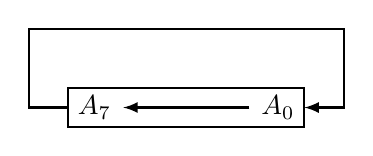
\begin{tikzpicture}
\def\kA{3}
\def\kB{0.5}
\draw[thick](0,-0.5*\kB)rectangle++(\kA,\kB);
\draw(0,0)node[right]{$A_7$} (\kA,0)node[left]{$A_0$};
\draw[-latex,thick](0,0)--++(-0.5,0)--++(0,1)--++(\kA+1,0)--++(0,-1)--++(-0.5,0);
\draw[-latex,thick](2.3,0)--(0.7,0);
\end{tikzpicture}
\caption{}
\end{subfigure}%
\begin{subfigure}{0.45\textwidth}
\centering
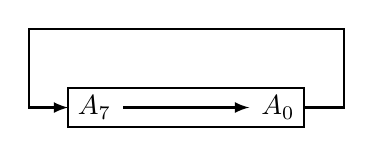
\begin{tikzpicture}
\def\kA{3}
\def\kB{0.5}
\draw[thick](0,-0.5*\kB)rectangle++(\kA,\kB);
\draw(0,0)node[right]{$A_7$} (\kA,0)node[left]{$A_0$};
\draw[latex-,thick](0,0)--++(-0.5,0)--++(0,1)--++(\kA+1,0)--++(0,-1)--++(-0.5,0);
\draw[latex-,thick](2.3,0)--(0.7,0);
\end{tikzpicture}
\caption{}
\end{subfigure}
\caption{گھوم ہدایات: (ا)\sRAL؛ (ب) \sRAR}
\label{شکل_کمپیوٹر_با_گھوم_ہدایت}
\end{figure}
%
\begin{center}
\begin{tabular}{l}
\regA\,=\,\LR{1011\,0100}
\end{tabular}
\end{center}
ہدایت \sRAL کی تعمیل کے بعد درج ذیل ہو گا۔
\begin{center}
\begin{tabular}{l}
\regA\,=\,\LR{0110\,1001}
\end{tabular}
\end{center}
 آپ دیکھ سکتے ہیں کہ، ہر بِٹ ایک  قدم بائیں  لیتا ہے اور بلند تر رتبی بِٹ گھوم کر کمتر رتبی بِٹ کا مقام لیتا ہے۔

\جزوحصہء{\sRAR}
یہ ہدایت کہتی ہے  \قول{ دفتر \دفترالف کو  دائیں گھما}۔ اس مرتبہ دفتر \دفترالف کے تمام بِٹ ایک قدم دائیں لیتے ہیں اور کمتر رتبی بِٹ گھوم کر بلند تر رتبی بِٹ کے مقام پر جاتا ہے (شکل  \حوالہ{شکل_کمپیوٹر_با_گھوم_ہدایت}-ب  دیکھیں)۔ یوں درج ذیل صورت میں
\begin{center}
\begin{tabular}{l}
\regA\,=\,\LR{1011\,0100}
\end{tabular}
\end{center}
ہدایت \sRAR کی تعمیل کے بعد درج ذیل ہو گا۔
\begin{center}
\begin{tabular}{l}
\regA\,=\,\LR{0101\,1010}
\end{tabular}
\end{center}

%---------------------------
%ex 11.13
\ابتدا{مثال}
بائٹ میں بِٹوں کی گنتی (کم تر  رتبی تا بلند  تر رتبی) \عددی{0} تا \عددی{7}  کی جاتی ہے۔ ایک برنامہ لکھیں جو روزن \عددی{2} سے بائٹ لے کر معلوم کرے آیا بِٹ \عددی{0} بلند یا پست ہے۔ بلند بِٹ کی صورت میں دفتر \دفترالف میں   لاطینی حرف \عددی{Y} کا ، اور پست بِٹ کی صورت میں  \عددی{N} کا ایسکی رمز ڈال کر روزن \عددی{3}  سے برآمد کریں۔

حل:\quad
\begin{center}
\begin{tabular}{rrr}
\toprule
سرخی&\multicolumn{1}{c}{ہدایت}&\multicolumn{1}{c}{تبصرہ}\\[1ex]
&\IN{\kop{02H}}& ؛ روزن \عددی{2} سے بائٹ لیں\\
&\ANI{\kop{01H}}& ؛ بِٹ \عددی{0} علیحدہ کریں\\
&\JNZ{ہاں}&؛ بلند بِٹ کی صورت میں شاخ لیں\\
&\MVI{\regA}{\kop{4EH}}& ؛ پست بِٹ کی صورت میں \عددی{N} ہو گا\\
&\JMP{اختتام}&؛ اگلی ہدایت نظر انداز کریں\\
ہاں:&\MVI{\regA}{\kop{59H}}& ؛ بلند بِٹ کی صورت میں \عددی{Y} ہو گا\\
اختتام:&\OUT{\kop{03H}}& ؛ روزن \عددی{3} پر  نتیجہ خارج کریں\\
&\HLT
\end{tabular}
\end{center}

روزن \عددی{2} سے دفتر \دفترالف میں( درج ذیل  روپ   کا) مواد داخل کیا جاتا ہے۔
\begin{center}
\begin{tabular}{l}
\regA\,=\,$A_7A_6A_5A_4A_3A_2A_1A_0$
\end{tabular}
\end{center}
ہدایت \عددی{\ANI{\kop{01H}}} میں متصل بائٹ درج ذیل ہے
\begin{center}
\begin{tabular}{l}
\LR{0000\,0001}
\end{tabular}
\end{center}
جس کو  \اصطلاح{نقاب}\فرہنگ{نقاب}\حاشیہب{mask}\فرہنگ{mask}  کہتے ہیں۔ اس بائٹ میں پست  \عددی{(0)} بِٹ،   دفتر \دفترالف کے مطابقتی  بلند  بِٹ نقاب پوش کر کے   پست کرتے ہیں۔ دوسرے لفظوں میں،  \sANI{01H} کی تعمیل کے بعد دفتر \دفترالف میں درج ذیل ہو گا۔
\begin{center}
\begin{tabular}{l}
\regA\,=\, \LR{$0000\, 000A_0$}
\end{tabular}
\end{center}

اگر \عددی{A_0} بلند \عددی{(1)}  ہو، \sJNZ شاخ کرتے ہوئے \MVI{\regA}{59H} کو پہنچے گا؛ جو  دفتر \دفترالف میں  \عددی{Y} کا ایسی رمز \عددی{59H} ڈالتا ہے۔ اگر \عددی{A_0} پست ہو، برنامہ \MVI{\regA}{4EH}  سے سیدھا گزرتے ہوئے، دفتر \دفترالف میں \عددی{N} کا ایسکی رمز ڈالتا ہے۔

ہدایت \OUT{03H} دفتر \دفترالف کا مواد روزن \عددی{3} سے خارج کرتا ہے۔ یوں  ثنائی تختی پر  \عددی{59H} یا \عددی{4EH} نظر آئے گا۔
\انتہا{مثال}
%-----------------------------------
%ex 11.14
\ابتدا{مثال}
متوازی  مخارج  کی بجائے ہم  روزن \عددی{4} سے مواد  سلسلہ وار    برآمد کرنا چاہتے ہیں۔  مذکورہ بالا برنامے میں تبدیلی پیدا کرتے ہوئے جواب (\عددی{59H} یا \عددی{4EH}) روزن \عددی{4} کے بِٹ \عددی{0} سے  سلسلہ وار خارج کریں۔

حل:\quad
\begin{center}
\begin{tabular}{rrr}
\toprule
سرخی&\multicolumn{1}{c}{ہدایت}&\multicolumn{1}{c}{تبصرہ}\\[1ex]
&\IN{\kop{02H}}&\\
&\ANI{\kop{01H}}&\\
&\JNZ{ہاں}&\\
&\MVI{\regA}{\kop{4EH}}&\\
&\JMP{ہوگیا}&\\
ہاں:&\MVI{\regA}{\kop{59H}}&\\
ہوگیا:&\MVI{\regC}{08H}& ؛ گنتکار میں \عددی{8} ڈالیں\\
دوبارہ:& \OUT{04H} & ؛ کمتر رتبی بِٹ خارج کریں\\
&\RAR& ؛ اگلی بِٹ تیار کریں\\
&\DCR{\regC}& ؛ گنتکار گھٹائیں\\
&\JNZ{دوبارہ} & ؛ گنتی پر نظر رکھیں\\
&\HLT
\end{tabular}
\end{center}

مواد کو متوازی سے سلسلہ وار   بنا کر ، بِٹ \عددی{A_0} سے  پہلے  بھیجا جاتا ہے؛ اس کے بعد  \عددی{A_1}، اور اس کے بعد \عددی{A_2}؛ اسی طرح چلتے ہوئے بِٹ \عددی{A_7}    سب سے آخر میں خارج کیا جاتا ہے۔
\انتہا{مثال}
%------------------------------
%ex 11.15
\ابتدا{مثال}
برآمد اور درآمد کے دوران خرد عامل کار    اور  (اس کے ساتھ جڑے ) بیرونی    آلے   کے بیچ تبادلے  (بات چیت ) کو\اصطلاح{ مصافحہ }\فرہنگ{مصافحہ}\حاشیہب{handshaking}\فرہنگ{handshaking} کہتے ہیں۔

کمپیوٹر با میں  مصافحہ  درج ذیل صورت اختیار کرتا ہے۔
جب آپ شکل   \حوالہ{شکل_کمپیوٹر_با_تعمیر} کے سادس عشری  مرموز کار میں دو اعداد (ایک بائٹ)  داخل کرتے ہیں، یہ مواد روزن \عددی{1} میں ڈالا جاتا ہے؛ ساتھ ہی روزن \عددی{2} کو بلند \قول{تیار}   اشارہ بھیجا جاتا ہے۔

داخلی مواد قبول کرنے سے قبل، خرد عامل کار روزن \عددی{2}   میں \قول{تیار} اشارے کو دیکھتا ہے۔ اگر  \قول{تیار}  اشارہ پست ہو، خرد عامل کار انتظار کرے گا۔ اگر \قول{تیار} بلند ہو، خرد عامل کار مواد قبول کر کے روزن \عددی{1} میں ڈالتا ہے۔ مواد کی ترسیل مکمل ہونے پر خرد عامل کار  ، سادس عشری ٹائپ کار  کے  مرموز کار  کو  \قول{تشکر} اشارہ بھیجتا ہے؛ جس کی بدولت \قول{تیار} بِٹ پست   کر دیا جائے گا۔ \قول{تشکر} بِٹ اس کے بعد پست کر دیا جاتا ہے۔

ٹائپ کار تختی پر نیا بائٹ  لکھنے پر یہی  عمل دوبارہ  کیا جائے گا؛ روزن \عددی{2}  کو \قول{تیار} اشارہ بھیجا جائے گا اور نیا مواد روزن \عددی{1} میں ڈالا جائے گا۔

کمپیوٹر با کا مصافحہ  درج ذیل اقدام  پر مشتمل ہے۔
\begin{enumerate}[1.]
\item
\قول{تیار} بِٹ (روزن \عددی{2} کا بِٹ \عددی{0}) بلند  ہو گا۔
\item
خرد عامل کار کے روزن \عددی{1} میں مواد  داخل ہو گا۔
\item
ر \قول{تیار} بِٹ پست کرنے کی خاطر \قول{تشکر} بِٹ (روزن \عددی{4} کا بِٹ \عددی{7} )  بلند ہو گا۔
\item
\قول{تشکر} بِٹ پست ہو گا۔

\end{enumerate}

مصافحہ استعمال کر کے روزن \عددی{1} سے ایک بائٹ مواد  درآمد کریں۔ اس بائٹ کو دفتر \دفترب میں ڈالیں۔

حل:\quad
\begin{center}
\begin{tabular}{rrr}
\toprule
سرخی&\multicolumn{1}{c}{ہدایت}&\multicolumn{1}{c}{تبصرہ}\\[1ex]
کیفیت:& \IN{02H} &؛ روزن \عددی{2} سے بائٹ لیں\\
&\ANI{01H}& ؛ تیار بِٹ کو علیحدہ کریں\\
&\JZ{کیفیت}& ؛ تیار نہ ہونے کی صورت میں انتظار کریں\\
&\IN{01H}& ؛ روزن \عددی{1} میں  بائٹ لیں\\
&\MOV{\regB}{\regA}& ؛ دفتر \دفترالف سے مواد دفتر\دفترب میں ڈالیں\\
&\MVI{\regA}{80H}& ؛ تشکر کا بِٹ بلند کریں\\
&\OUT{04H}& ؛ بلند تشکر خارج کریں\\
&\MVI{\regA}{00H}&؛ تشکر بِٹ پست کریں\\
&\OUT{04H}&؛ پست تشکر خارج کریں\\
&\HLT
\end{tabular}
\end{center}

اگر \قول{تیار} بِٹ پست ہو \ANI{01H} کی تعمیل دفتر \دفترالف کے مواد کو صفر بنائے گی جس سے جھنڈا صفر بلند ہو گا۔ یوں \JZ{کیفیت}ہدایت واپس       دائرے کے  آغاز میں \IN{02H} کو شاخ  کرے گی۔جب تک \قول{تیار} بِٹ بلند نہ ہو،کمپیوٹر  دائرے  میں رہے گا۔

بلند \قول{تیار} اشارہ درست مواد کی تصدیق کرتا ہے۔  بلند \قول{تیار} بِٹ کی صورت میں  برنامہ \sJZ سے گزر کر \IN{02H} پہنچے گا۔ یوں روزن \عددی{1} سے دفتر \دفترالف میں بائٹ منتقل ہو گا۔ \sMOV اس بائٹ کو دفتر \دفترب منتقل کرتی ہے۔ ہدایت \MVI{\regA}{80H} \قول{تشکر} بِٹ (بِٹ \عددی{7}) بلند کرتی ہے۔ \OUT{04H} ہدایت بلند  \قول{تشکر}  اشارہ  سادس عشری مرموز کار کو بھیجتی ہے ، جس کا اندرونی سخت افزار  \قول{تیار} بِٹ پست کرتا ہے۔ اس کے بعد \قول{تشکر} بِٹ پست کیا جاتا ہے تا کہ اگلا بِٹ درآمد کرنا ممکن ہو۔
\انتہا{مثال}
%------------------------

\حصہ{کمپیوٹر با کا خلاصہ}
اس حصے میں کمپیوٹر با کے \عددی{T} حال، جھنڈے، اور  پتہ نشر کرنے کے انداز پر غور کیا جائے گا۔

\جزوحصہء{\عددی{T} حال}
کمپیوٹر با کا قابو و ترتیب کار کا برنامہ  متغیر مشینی پھیرے کے لئے   ہے۔ یوں بعض ہدایات کی تعمیل باقی ہدایات کی تعمیل سے  زیادہ  لے گی۔ جیسا آپ کو یاد ہو گا، خرد برنامہ نویسی کا مقصد پختہ حافظہ میں قابو  معمولے ذخیرہ کرنا ہے، جہاں سے انہیں ضرورت کے پیش  اٹھایا جا سکتا ہے۔

جدول  \حوالہ{جدول_کمپیوٹر_با_ہدایات_اور_ٹی_حال}  میں  ہر ایک ہدایت  اور ہدایت کی تعمیل کے لئے درکار \عددی{T} حال کی تعداد پیش ہے۔ مثلاً، \ADD{\regB} کی تعمیل چار \عددی{T} حال میں ہو گی، \ANI{بائٹ} کی تعمیل  سات میں،  اور \sCALL کی اٹھارہ میں، وغیرہ۔ وقتیہ استعمال میں \عددی{T} حال کی تعداد جاننا ضروری ہو گا۔

دھیان رہے کہ \sJM کو  درکار \عددی{T} حال  کی تعداد \عددی{10/7} ہے۔شاخ لینے کی صورت میں درکار  \عددی{T} حال کی تعداد \عددی{10} اور سیدھا گزرنے کی صورت میں \عددی{7} ہے۔ یہی تصور باقی مشروط شاخ ہدایات کے لئے بھی  ہے؛ شاخ  کی صورت میں درکار \عددی{T} حال کی تعداد  \عددی{10}  اور شاخ نہ لینے کی صورت میں \عددی{7} ہو گی۔

\begin{table}
\caption{کمپیوٹر با کی ہدایات کا سلسلہ}
\label{جدول_کمپیوٹر_با_ہدایات_اور_ٹی_حال}
\centering
\begin{tabular}{rccrrr}
\toprule
ہدایت& ہدایتی رمز& \عددی{T} حال& \multicolumn{1}{c}{جھنڈے}&انداز پتہ&\multicolumn{1}{c}{بائٹ}\\
\midrule
\ADD{\regB}&80&4&S ، \,Z & دفتری&1\\
\ADD{\regC}&81&4&S ، \,Z&دفتری&1\\
\ANA{\regB}&A0&4&S ، \,Z&دفتری&1\\
\ANA{\regC}&A1&4&S ، \,Z&دفتری&1\\
\ANI{بائٹ}&E6&7&S ، \,Z&متصل&2\\
\CALL{پتہ}&CD&18&کوئی نہیں& متصل&3\\
\CMA&2F&4&کوئی نہیں&مضمر&1\\
\DCR{\regA}&3D&4& S ، \,Z&دفتری&1\\
\DCR{\regB}&05&4&S ، \,Z&دفتری&1\\
\DCR{\regC}&0D&4&S ، \,Z&دفتری&1\\
\HLT&76&5&کوئی نہیں&کوئی نہیں&1\\
\IN{بائٹ}&DB&10&کوئی نہیں&بلاواسطہ&2\\
\INR{\regA}&3C&4&S ، \,Z&دفتری&1\\
\INR{\regB}&04&4&S ، \,Z&دفتری&1\\
\INR{\regC}&0C&4&S ، \,Z&دفتری&1\\
\JM{پتہ}&FA&10/7&کوئی نہیں&متصل&3\\
\JMP{پتہ}&C3&10&کوئی نہیں&متصل&3\\
\JNZ{پتہ}&C2&10/7&کوئی نہیں&متصل&3\\
\JZ{پتہ}&CA&10/7&کوئی نہیں&متصل&3\\
\LDA{پتہ}&3A&13&کوئی نہیں&بلاواسطہ&3\\
\MOV{\regA}{\regB}&78&4&کوئی نہیں&دفتری&1\\
\MOV{\regA}{\regC}&79&4&کوئی نہیں&دفتری&1\\
\MOV{\regB}{\regA}&47&4&کوئی نہیں&دفتری&1\\
\MOV{\regB}{\regC}&41&4&کوئی نہیں&دفتری&1\\
\MOV{\regC}{\regA}&4F&4&کوئی نہیں&دفتری&1\\
\MOV{\regC}{\regB}&48&4&کوئی نہیں&دفتری&1\\
\MVI{\regA}{بائٹ}&3E&7&کوئی نہیں&متصل&2\\
\MVI{\regB}{بائٹ}&06&7&کوئی نہیں&متصل&2\\
\MVI{\regC}{بائٹ}&0E&7&کوئی نہیں&متصل&2\\
\NOP&00&4&کوئی نہیں&کوئی نہیں&1\\
\ORA{\regB}&B0&4&S ، \,Z&دفتری&1\\
\ORA{\regC}&B1&4&S ، \,Z&دفتری&1\\
\ORI{بائٹ}&F6&7&S ، \,Z&متصل&2\\
\OUT{بائٹ}&D3&10&کوئی نہیں&بلاواسطہ&2\\
\RAL&17&4&کوئی نہیں&مضمر&1\\
\RAR&1F&4&کوئی نہیں&مضمر&1\\
\RET&C9&10&کوئی نہیں&مضمر&1\\
\STA{پتہ}&32&13   &کوئی نہیں&بلاواسطہ&3\\
\SUB{\regB}&90&4&S ، \,Z&دفتری&1\\
\SUB{\regC}&91&4&S ، \,Z&دفتری&1\\
\XRA{\regB}&A8&4&S ، \,Z&دفتری&1\\
\XRA{\regC}&A9&4&S ، \,Z&دفتری&1\\
\XRI{بائٹ}&EE&7&S ، \,Z&متصل&2\\
\bottomrule
\end{tabular}
\end{table}

\جزوحصہء{جھنڈے}
جیسا آپ جانتے ہیں، بعض ہدایات کی تعمیل کے دوران دفتر \دفترالف منفی   یا  صفر ہو   سکتا ہے، جس سے  بالترتیب جھنڈا منفی اور جھنڈا  صفر اثر انداز ہوں گے۔ شکل \حوالہء{11.8} میں کمپیوٹر با کے جھنڈے   بلند کرنے کے ادوار پیش ہیں۔

دفتر \دفترالف کا مواد منفی ہونے کی صورت میں  \عددی{A_7}   بِٹ \عددی{1} ہو گا۔ یہ علامت بِٹ زیریں ضرب  گیٹ کو چلاتی ہے۔  جب دفتر کا مواد صفر ہو، تمام بِٹ پست ہوں گے، اور جمع متمم گیٹ کا مخارج بلند \عددی{(1)}  ہو گا۔اس  جمع متمم  گیٹ کا مخارج بالا ضرب گیٹ کو چلاتا ہے۔ اگر \عددی{L_F}  بلند ہو،   جھنڈے ان نتائج کے تحت   صورت اختیار کر کے دفتر \دفترالف  کی  علامت اور صفر صورت  کا عکس پیش کریں گے۔ یوں دفتر \دفترالف کا مواد منفی ہونے کی صورت میں \عددی{S} بلند ہو گا، اور مواد صفر ہونے کی صورت میں \عددی{Z} بلند ہو گا۔

ایسا نہیں کہ تمام ہدایات جھنڈوں پر اثر انداز ہوتی ہیں۔ جیسا جدول  \حوالہ{جدول_کمپیوٹر_با_ہدایات_اور_ٹی_حال} میں دکھایا گیا ہے \sADD، \sANA، \sANI، \sDCR، \sINR، \sORA، \sSUB، \sXRA، اور \sXRI وہ ہدایات ہیں جو جھنڈوں پر اثر انداز ہوتی ہیں۔ صرف یہ ہدایات کیوں؟  اس لئے کہ شکل \حوالہء{11.8} میں \عددی{L_F} اشارہ صرف اس وقت بلند ہو گا جب ان  ہدایات  کی تعمیل ہو۔  ان ہدایات کے لئے \عددی{L_F} بِٹ کی  خرد برنامہ نویسی سے یہ ممکن بنایا جاتا ہے۔ دوسرے لفظوں میں، قابو پختہ حافظہ میں ہم مذکورہ بالا ہدایات کے لئے \عددی{L_F} بِٹ  بلند   رکھتے ہیں، جبکہ باقی ہدایات کے لئے  ہم \عددی{L_F} بِٹ  پست رکھتے ہیں۔

\جزوحصہء{مشروط شاخ}
جیسا ذکر کیا گیا، شاخ لینے کی صورت میں مشروط  شاخ ہدایات  دس \عددی{T} حال، جبکہ سیدھا گزرنے کی صورت میں سات \عددی{T} حال لیتے ہیں۔اس کی وجہ  مختصراً درج ذیل ہے۔ تعمیلی پھیرے کے دوران پتہ پختہ حافظہ ،  کمپیوٹر کو مشروط شاخ کے    خرد معمولہ کی پہلی ہدایت کے پتے پر بھیجتا ہے۔ خرد معمولہ  کا ابتدائی حصہ جھنڈے کو  پرکھ  کر شاخ لینے یا نہ لینے کا فیصلہ کرتا ہے۔ اگر شاخ لینا مقصود ہو، خرد معمولہ کا باقی حصہ زیر  عمل آئے گا؛ دیگر صورت  خرد معمولہ کا  باقی حصہ رد کیا جاتا ہو اور کمپیوٹر  سیدھا گزر کر اگلی ہدایات اٹھاتا  ہے۔

\جزوحصہء{پتہ نشر کرنے کے انداز}
کمپیوٹر با کی ہدایات  مختلف طریقوں سے  مواد تک رسائی حاصل کرتی ہیں۔ رقم زیر عمل  ہمیں بتاتا  ہے کہ  مواد تک رسائی کس طرح حاصل کرنی ہے۔ مثال کے طور پر،  درج ذیل ہدایات میں مواد کا پتہ فراہم کیا گیا ہے۔
\begin{center}
\begin{tabular}{r}
\LDA{پتہ}\\
\STA{پتہ}
\end{tabular}
\end{center}
یہ\اصطلاح{ بلا واسطہ پتے  کا انداز}\فرہنگ{پتہ!بلا واسطہ انداز}\حاشیہب{direct addressing}\فرہنگ{addressing!direct} کی مثال ہیں۔

\اصطلاح{متصل پتے کا انداز}\فرہنگ{پتہ!متصل انداز}\حاشیہب{immediate addressing}\فرہنگ{addressing!immediate} فراہم کرنے کا انداز   اس سے مختلف ہے۔ مواد کا پتہ فراہم کرنے کی بجائے، ہم مواد فراہم کرتے ہیں۔ مثلاً، درج ذیل ہدایت میں  درکار بائٹ  ،  حافظہ میں ہدایتی رمز کے فوراً بعد   پایا جاتا ہے۔
\begin{center}
\begin{tabular}{r}
\MVI{\regA}{بائٹ}
\end{tabular}
\end{center}
جدول \حوالہ{جدول_کمپیوٹر_با_ہدایات_اور_ٹی_حال} میں متصل پتہ کے   دیگر  ہدایات پیش ہیں۔

درج ذیل ہدایت  میں  مطلوبہ مواد، حافظہ کی بجائے  دفتر میں پایا جاتا ہے۔ یہ\اصطلاح{ دفتری پتہ  انداز}\فرہنگ{پتہ!دفتری انداز}\حاشیہب{register addressing}\فرہنگ{addressing!register} کی مثال ہے۔
\begin{center}
\begin{tabular}{r}
\MOV{\regA}{\regB}
\end{tabular}
\end{center}
دفتری  پتہ کے  انداز میں \عددی{T} حال  کی تعداد کم ہے  لہٰذا یہ  نہایت چست ہدایات دیتی ہیں۔

\اصطلاح{مضمر پتہ کا انداز }\فرہنگ{پتہ!مضمر انداز}\حاشیہب{implied addressing}\فرہنگ{addressing!implied}  میں مواد کا پتہ ہدایت کے اندر موجود ہو گا۔ مثال کے طور پر،
\begin{center}
\begin{tabular}{r}
\RAL
\end{tabular}
\end{center}
کہتی ہے دفتر \دفترالف کے  بِٹ  بائیں  گھمائیں۔ مواد دفتر \دفترالف میں موجود ہے؛ یہی وجہ ہے کہ مضمر پتے کے انداز میں رقم زیر عمل کی ضرورت نہیں ہوگی۔

\جزوحصہء{بائٹ}
 ہدایت کو  حافظہ میں رکھنے کے لئے  ایک یا ایک سے زیادہ بائٹ کی جگہ درکار ہو گی۔کمپیوٹر با کی ہدایات  کو \عددی{1}، \عددی{2}، یا \عددی{3} بائٹ جگہ چاہیے ہو گی۔ جدول \حوالہ{جدول_کمپیوٹر_با_ہدایات_اور_ٹی_حال} میں ہر ہدایت کو درکار بائٹ  بتائے  گئے ہیں۔ جیسا آپ دیکھ سکتے ہیں، \sADD ہدایت کو \عددی{1} بائٹ، \sANI ہدایت کو \عددی{2}  بائٹ، اور \sCALL ہدایت کو \عددی{3} بائٹ جگہ چاہیے، وغیرہ۔
 
 %----------------------------------
 %ex 11.16
 \ابتدا{مثال}
 کمپیوٹر با کی ساعت کا تعدد \عددی{\SI{1}{\mega\hertz}} ہے۔ یوں ایک \عددی{T} حال کا دورانیہ \عددی{\SI{1}{\micro\second}} ہو گا۔ درج ذیل ذیلی معمولہ کی تعمیل کتنی دیر میں ہو گی؟
 \begin{center}
\begin{tabular}{rrr}
\toprule
سرخی&\multicolumn{1}{c}{ہدایت}&\multicolumn{1}{c}{تبصرہ}\\[1ex]
&\MVI{\regC}{46H}&؛ گنتکار  عشری \عددی{70} رکھیں\\
دوبارہ:&\DCR{\regC}& ؛ نیچے شمار کریں\\
&\JNZ{دوبارہ}&؛ گنتی پرکھیں\\
&\NOP&؛ مزید وقفہ دیں\\
&\RET&
\end{tabular}
\end{center}

حل:\quad
گنتکار کی ابتدائی قیمت تعین کرنے کی خاطر  \sMVI ہدایت  کی تعمیل ایک مرتبہ کی جاتی ہے۔ ہدایت \sDCR کی تعمیل \عددی{70} مرتبہ ہو گی۔  ہدایت \sJNZ پورے \عددی{69} مرتبہ شاخ لی گی اور ایک مرتبہ سیدھا گزرنے دے گی۔ جدول \حوالہ{جدول_کمپیوٹر_با_ہدایات_اور_ٹی_حال} میں \عددی{T} حال   کی تعداد پیش ہے، جنہیں استعمال کر کے  ذیلی معمولہ کی تعمیلی دورانیہ معلوم کرتے ہیں۔
\begin{center}
\begin{tabular}{rrr}
\sMVI&\(1\times 7\times \SI{1}{\micro\second}=\SI{7}{\micro\second}\)&\\
\sDCR&\(70\times 4\times \SI{1}{\micro\second}=\SI{280}{\micro\second}\)&\\
\sJNZ&\(69\times 10\times \SI{1}{\micro\second}=\SI{690}{\micro\second}\)&(شاخ لیا گیا)\\
\sJNZ&\(1\times 7\times \SI{1}{\micro\second}=\SI{7}{\micro\second}\)&(شاخ نہیں لیا گیا)\\
\sNOP&\(1\times 4\times \SI{1}{\micro\second}=\SI{4}{\micro\second}\)&\\
\sRET&\(1\times 10\times \SI{1}{\micro\second}=\SI{10}{\micro\second}\)&
\end{tabular}
\end{center}
یوں درکار وقت \عددی{7+280+690+7+4+10=\SI{998}{\micro\second}} ہو گا، جو تقریباً  \عددی{\SI{1}{\milli]second}} کے برابر ہے۔

اس ذیلی معمولہ کو طلب کر کے \عددی{\SI{1}{\milli\second}} کا وقفہ پیدا کیا جا سکتا ہے۔ 

جدول \حوالہ{جدول_کمپیوٹر_با_ہدایات_اور_ٹی_حال} کے تحت اس ذیلی معمولہ میں مستعمل ہدایات کی لمبائی درج ذیل ہے۔
\begin{center}
\begin{tabular}{r|ccccc}
ہدایت&
\sMVI&\sDCR&\sJNZ&\sNOP&\sRET\\
\midrule
بائٹ&
2&1&3&1&1
\end{tabular}
\end{center}

اس معمولہ کی کل  لمبائی  \عددی{8} بائٹ ہے۔ کمپیوٹر با کے نرم افزار کے طور پر اس معمولہ    کا ترجمہ مشینی زبان میں کر کے  \عددی{F010H} تا \عددی{F017H} پتے  پر رکھا جا سکتا ہے۔ ایسا کرنے کے بعد، \CALL{F010H} ہمیں \عددی{\SI{1}{\milli\second}} وقفہ  دیگا۔
 \انتہا{مثال}
 %---------------------------
 %ex 11.17

 \ابتدا{مثال}
 درج ذیل معمولہ کتنا وقفہ پیدا کرتا ہے؟
\begin{center}
\begin{tabular}{rrr}
\toprule
سرخی&\multicolumn{1}{c}{ہدایت}&\multicolumn{1}{c}{تبصرہ}\\[1ex]
&\MVI{\regB}{0AH}& ؛ گنتکار  \دفترب عشری \عددی{10}ہے\\
دائرہ1:&
\MVI{\regC}{47H}&؛ گنتکار \دفترج عشری  \عددی{71} رکھیں\\
دائرہ2:&
\DCR{\regC}&؛ \دفترج گھٹائیں\\
&\JNZ{دائرہ2}&؛ \دفترج صفر ہونے پر نظر رکھیں\\
&\DCR{\regB}&؛ \دفترب گھٹائیں\\
&\JNZ{دائرہ1}& ؛ \دفترب صفر ہونے پر نظر رکھیں\\
&\RET&
\end{tabular}
\end{center}

حل:\quad
اس ذیلی معمولہ  میں دو دائرے ہیں۔ بیرونی دائرے کو دائرہ1 کہا گیا ہے؛ اندرونی کو دائرہ2 کہا گیا ہے۔ اندرونی دائرہ \DCR{\regC} اور \JNZ{دائرہ2} ہدایات پر مشتمل ہے۔ اندرونی دائرہ  \عددی{\SI{991}{\micro\second}} کا وقفہ پیدا کرتا ہے، جس کی تفصیل ذیل ہے۔
\begin{center}
\begin{tabular}{rrr}
\sDCR&\(71\times 4\times \SI{1}{\micro\second}=\SI{284}{\micro\second}\)&\\
\sJNZ&\(70\times 10\times \SI{1}{\micro\second}=\SI{700}{\micro\second}\)&(شاخ لیا گیا)\\
\sJNZ&\(1\times 7\times \SI{1}{\micro\second}=\SI{7}{\micro\second}\)&(شاخ نہیں لیا گیا)\\
\end{tabular}
\end{center}
جب گنتکار \دفترج  صفر کو پہنچتا ہے ، برنامہ \JNZ{دائرہ2} سے نیچے  گرتا ہے؛ گنتکار \دفترب گھٹتا ہے اور \JNZ{دائرہ1} ہدایت،   برنامے کو واپس \MVI{\regC}{47H} بھیجتی ہے۔ ہم دائرہ2 میں دوسری مرتبہ داخل ہوتے ہیں۔ چونکہ دائرہ1 کے اندر دائرہ2 پایا جاتا ہے لہٰذا  دائرہ2 کی تعمیل \عددی{10} مرتبہ ہو گی اور یوں کل وقفہ  تقریباً \عددی{\SI{10}{\milli\second}} پیدا ہو گا۔

پورے ذیلی معمولہ  کے حساب کی تفصیل درج ذیل ہے، جو  \عددی{\SI{10134}{\micro\second}} ( تقریباً \عددی{\SI{10}{\milli\second}} ) وقفہ دیتا   ہے۔
\begin{center}
\begin{tabular}{rrr}
\MVI{\regB}{0AH}&\(1\times 7\times \SI{1}{\micro\second}=\SI{7}{\micro\second}\)&\\
\MVI{\regC}{47H}&\(1\times 7\times \SI{1}{\micro\second}=\SI{7}{\micro\second}\)&\\
دائرہ2&
\(10\times \SI{991}{\micro\second}=\SI{9910}{\micro\second}\)&\\
\DCR{\regB}&\(10\times 4\times \SI{1}{\micro\second}=\SI{40}{\micro\second}\)&\\
\JNZ{دائرہ1}&\(9\times 10\times \SI{1}{\micro\second}=\SI{90}{\micro\second}\)&(شاخ لیا گیا)\\
\JNZ{دائرہ1}&\(1\times 7\times \SI{1}{\micro\second}=\SI{7}{\micro\second}\)&(شاخ نہیں لیا گیا)\\
\RET&\(1\times 10\times \SI{1}{\micro\second}=\SI{10}{\micro\second}\)&
\end{tabular}
\end{center}
اس ذیلی معمولہ کی لمبائی (\عددی{13} بائٹ)  درج ذیل   ہے۔
\begin{align*}
2+2+1+3+1+3+1=13
\end{align*}
اس ذیلی معمولہ  کا ترجمہ مشینی زبان میں کر کے \عددی{F020H} تا \عددی{F02CH} پتے پر رکھتے ہیں۔ایسا کرنے کے بعد، \CALL{F020H} ہدایت  ہمیں تقریباً \عددی{\SI{10}{\milli\second}} کا وقفہ دیگی۔

پہلی ہدایت کو تبدیل کر کے  درج ذیل بنانے سے گنتکار \دفترب میں عشری \عددی{100} ڈالا جائے گا۔
\begin{center}
\begin{tabular}{r}
\MVI{\regB}{64H}
\end{tabular}
\end{center}
اندرونی دائرے کی تعمیل \عددی{100} مرتبہ ہو گی، اور کل وقفہ  تقریباً \عددی{\SI{100}{\milli\second}} ہو گا۔ اس ذیلی معمولہ کو، جو \عددی{\SI{100}{\milli\second}} وقفہ دیتا ہے،  پتہ \عددی{F030H} تا \عددی{F03CH} پر رکھتے ہیں۔
 \انتہا{مثال}
 %--------------------------
 %ex11.18
 \ابتدا{مثال}
 درج ذیل ذیلی معمولہ\اصطلاح{  محیط  دائروں } \فرہنگ{محیط دائرے}\حاشیہب{nested loops}\فرہنگ{nested loops} پر مشتمل ہے جو ایک دوسرے کے  اندر  رکھے گئے  ہیں۔ یہ کتنا وقفہ پیدا  کرتا ہے؟
 
 حل:\quad
 \begin{center}
\begin{tabular}{rrr}
\toprule
سرخی&\multicolumn{1}{c}{ہدایت}&\multicolumn{1}{c}{تبصرہ}\\[1ex]
&\MVI{\regA}{0AH}&؛ گنتکار \دفترالف میں عشری \عددی{10} ڈالیں\\
دائرہ1&\MVI{\regB}{64H}& ؛ گنتکار  \دفترب عشری \عددی{100}ہے\\
دائرہ2:&
\MVI{\regC}{47H}&؛ گنتکار \دفترج عشری  \عددی{71} رکھیں\\
دائرہ3:&
\DCR{\regC}&؛ \دفترج گھٹائیں\\
&\JNZ{دائرہ3}&؛ \دفترج صفر ہونے پر نظر رکھیں\\
&\DCR{\regB}&؛ \دفترب گھٹائیں\\
&\JNZ{دائرہ2}& ؛ \دفترب صفر ہونے پر نظر رکھیں\\
&\DCR{\regA}&؛ گنتکار \دفترالف گھٹائیں\\
&\JNZ{دائرہ1}& ؛\دفترالف کو صفر کے لئے پرکھیں\\
&\RET&
\end{tabular}
\end{center}
حل:\quad
دائرہ3 سے گزر تقریباً \عددی{\SI{1}{\milli\second}} میں ہو گی۔ دائرہ3 سے دائرہ2  سو مرتبہ گرتا ہے  جو تقریباً \عددی{\SI{100}{\milli\second}} میں ہو گا۔ دائرہ2 سے دائرہ1 پورے دس مرتبہ گزرتا ہے، جو تقریباً ایک سیکنڈ \عددی{(\SI{1}{\second})} لیگا۔ یوں ذیلی معمولہ کل ایک سیکنڈ وقفہ پیدا کرتا ہے۔

کیا آپ دیکھ سکتے ہیں، ہم کہاں جا رہے ہیں؟ ہم نے ایک سیکنڈ کا ذیلی معمولہ حاصل کر لیا ہے۔ اس کو \عددی{F040H} تا \عددی{F052H} پتے پر رکھتے ہیں۔ ایک سیکنڈ وقفہ پیدا کرنے کے لئے ہم \عددی{\CALL{F040H}} ہدایت استعمال کریں گے۔

اول ہدایت کو تبدیل کر کے درج ذیل بنانے سے دائرہ2 سے دائرہ1 سو مرتبہ گزرتا ہے، جو خود دائرہ0 سے سو مرتبہ گزرتا ہے۔حاصل ذیلی معمولہ  دس سیکنڈ کا وقفہ دیگا۔
 \begin{center}
\begin{tabular}{r}
\MVI{\regA}{64H}
\end{tabular}
\end{center}
اس کو \عددی{F060H} تا \عددی{F072H} پتے پر رکھتے ہیں۔ اس ذیلی معمولہ کو طلب کرنے سے \عددی{10} سیکنڈ کا وقفہ حاصل ہو گا۔

جدول  \حوالہ{جدول_کمپیوٹر_با_دورانے} میں کمپیوٹر با کے وقتی دورانیے پیش ہیں۔ انہیں استعمال کر کے \عددی{\SI{1}{\milli\second}} تا \عددی{\SI{10}{\second}} وقفے حاصل ہوں گے۔
 \انتہا{مثال}
 %----------------------------
 
 \begin{table}
 \caption{کمپیوٹر با کے ذیلی معمولے}
 \label{جدول_کمپیوٹر_با_دورانے}
 \centering
 \begin{tabular}{rrlr}
 \toprule
 سرخی&ابتدائی پتہ& وقفہ&مستعمل دفاتر\\
 \midrule
 وق1م&F010H&\(\SI{1}{\milli\second}\) &\regC\\
 وق10م&F020H&\(\SI{10}{\milli\second}\) &\regB، \regC\\
 وق100م&F030H&\(\SI{100}{\milli\second}\) &\regB، \regC\\
 وق1س&F040H&\(\SI{1}{\second}\) &\regA، \regB، \regC\\
 وق10س&F060H&\(\SI{10}{\second}\) &\regA، \regB، \regC\\
 \bottomrule
 \end{tabular}
 \end{table}
 
 %----------------------------------
 %ex11.19
 \ابتدا{مثال}
چوراہے  پر نسب \اصطلاح{ آمد و رفت بتی }\فرہنگ{آمد و رفت بتی}\حاشیہب{traffic lights}\فرہنگ{traffic lights} گاڑیوں کی حرکت قابو کرتی ہے۔ یہ بتی \عددی{\SI{50}{\second}} کے لئے سبز، \عددی{\SI{6}{\second}}  کے لئے پیلی، اور \عددی{\SI{30}{\second}}  کے لئے  لال   رہتی  ہے۔ روزن \عددی{4} کے بِٹ \عددی{1}، \عددی{2}، اور \عددی{3} بالترتیب   سبز، پیلی، اور لال    بلب  روشن کرنے والے ادوار کو جاتی ہیں۔   اس بتی کو چلانے کے لئے برنامہ لکھیں۔

حل:\quad
\begin{center}
\begin{tabular}{rrr}
\toprule
سرخی&\multicolumn{1}{c}{ہدایت}&\multicolumn{1}{c}{تبصرہ}\\[1ex]
دوبارہ:&
\MVI{\regA}{32H}&؛سبز بتی کو پچاس سیکنڈ کا وقفہ درکار ہے\\
&\STA{حفاظت}&؛ گنتکار\دفترالف کی موجودہ  گنتی  حفاظت سے رکھیں\\
&\MVI{\regA}{02H}&؛ بِٹ \عددی{1} بلند کر کے سبز بتی منتخب کریں\\
&\OUT{04H}&؛ سبز بتی روشن کریں\\
دائرہس:&
\CALL{وق1س}&؛ ایک سیکنڈ  ذیلی معمولہ طلب\\
&\LDA{حفاظت}&؛ گنتکار \دفترالف کی موجودہ گنتی  اٹھائیں\\
&\DCR{\regA}&؛ گنتکار \دفترالف گھٹائیں\\
&\STA{حفاظت}&؛ نئی گنتی کی حفاظت کریں\\
&\JNZ{دائرہس}& ؛ سبز بتی روشن رکھیں\\
&\MVI{\regA}{06H}&؛ پیلی بتی کو چھ سیکنڈ چاہیے\\
&\STA{حفاظت}&\\
&\MVI{\regA}{04H}&؛ بِٹ \عددی{2} بلند کر کے پیلی بتی کی نشاندہی کریں\\
&\OUT{04H}&پیلی بتی روشن کریں\\
دائرہپ:&
\CALL{وق1س}&\\
&\LDA{حفاظت}&\\
&\DCR{A}&\\
&\STA{حفاظت}&\\
&\JNZ{دائرہپ}&\\
&\MVI{\regA}{1EH}&؛ لال بتی \عددی{30} سیکنڈ روشن رہے گی\\
&\STA{حفاظت}&\\
&\MVI{\regA}{08H}&;لال بتی کا انتخاب کریں\\
&\OUT{04H}&؛ لال بتی روشن کریں\\
دائرہل:&
\CALL{وق1س}&\\
&\LDA{حفاظت}&\\
&\DCR{\regA}&\\
&\STA{حفاظت}&\\
&\JNZ{دائرہل}&\\
&\JMP{دوبارہ}&\\
حفاظت:&مواد&
\end{tabular}
\end{center}

آئیں   ذیلی معمولہ کے سبز بتی حصہ کو تفصیل سے دیکھیں؛ پیلی بتی اور لال بتی کے حصے بھی اسی طرح ہیں۔ آغاز \MVI{\regA}{32H}  ہدایت سے ہوتا ہے جو عشری \عددی{50} گنتکار \دفترالف میں ڈالتی ہے۔ دفتر \دفترالف دیگر  کاموں کے لئے   بھی مستعمل ہے لہٰذا اس میں موجود مواد کو \STA{حفاظت} حافظہ میں\قول{ حفاظت} پتے پر رکھتی ہے۔ ذیلی معمولہ کا آخری  مقام \قول{حفاظت}   کے لئے مختص ہے، جس کی نشاندہی  ذیلی معمولہ میں آخری سرخی  کرتی ہے۔ \MVI{\regA}{02H} دفتر \دفترالف کا بائٹ \عددی{1} بلند کرتی ہے، جو روزن \عددی{4} میں سبز بتی  کے لئے مختص ہے؛ \OUT{04H} روزن \عددی{4} کے بِٹ \عددی{1} کو بلند کرتی ہے، جو بیرونی دور کو سبز بتی روشن کرنے کا حکم ہے۔

جدول \حوالہ{جدول_کمپیوٹر_با_دورانے} میں ایک سیکنڈ وقفہ کے ذیلی معمولہ کا ابتدائی پتہ \عددی{F040H} دیا گیا ہے۔یوں ایک سیکنڈ وقفہ پیدا کرنے کے لئے ہم \عددی{\CALL{F040H}} لکھ سکتے ہیں، تاہم سرخی استعمال کرتے ہوئے اسی ذیلی معمولہ کو \CALL{وق1س} لکھ کر  طلب کیا جا سکتا ہے۔ ذیلی معمولہ کے ابتدائی مقام کو با  معنی   سرخی  سے منسوب کر کے پتہ کی بجائے استعمال کرنا  آسانی پیدا کرتا ہے۔

یوں  ہدایت \CALL{وق1س} ایک سیکنڈ وقفے کے ذیلی معمولہ کو طلب  کرتی ہے۔\LDA{حفاظت} گنتکار میں موجودہ گنتی ڈالتی ہے جو اس وقت  عشری \عددی{50} ہو گی۔ \DCR{\regA} اس گنتی کو گھٹا کر عشری \عددی{49} کرتی ہے۔ \STA{حفاظت}  نئی گنتی(عشری  \عددی{49} ) کا تحفظ کرتی ہے۔ اس کے بعد \JNZ{دائرہس} (دائرہ سبز چھوٹا کر کے\قول{ دائرہس } لکھا گیا ہے ، تا کہ سرخی پر عائد ، زیادہ سے زیادہ  چھ علامتوں کی شرط مطمئن  ہو)  مزید ایک سیکنڈ کا  وقفہ پیدا کرنے کے لئے واپس \CALL{وق1س} کو شاخ کرتی ہے۔

ہدایت \CALL{وق1س} پورا \عددی{50} مرتبہ طلب کیا گیا ہے؛ یوں سبز بتی \عددی{50} سیکنڈ روشن  رہتی ہے۔ اس کے بعد برنامہ \JNZ{دائرہس} سے نیچے گر کو  \MVI{\regA}{06H} پہنچتا ہے۔ یہاں سے پیلی بتی قابو کرنے حصہ  شروع ہوتا ہے۔ گنتکار \دفترالف میں عشری \عددی{6} ڈال کر ایک سیکنڈ وقفے کا ذیلی معمولہ  چھ مرتبہ طلب کیا جاتا ہے؛ یوں پیلی بتی \عددی{6} سیکنڈ روشن رہے گی۔

پیلی بتی کے بعد لال بتی کی باری آتی ہے۔ لال بتی  سے فارغ ہونے کے بعد \JMP{دوبارہ} ہدایت  برنامے کو نئے سرے  چلاتی ہے۔ یوں بتیاں مسلسل باری باری روشن ہوں گی۔
\انتہا{مثال}
%---------------------------
%ex 11.20
\ابتدا{مثال}
 مختلف صوتی تعدد   پیدا کرنے کے لئے  خرد عامل کار بروئے کار لایا  جا سکتا ہے۔ روزن \عددی{4} کا بِٹ \عددی{5}\اصطلاح{  افزائش کار}\فرہنگ{افزائش کار}\حاشیہب{amplifier}\فرہنگ{amplifier} (ایمپلی فائر)  کے ساتھ  جوڑا گیا ہے۔افزائش کار نا صرف برقی اشارہ مستحکم بناتا ہے بلکہ اس کا حیطہ بڑھانے کی صلاحیت بھی رکھتا ہے۔یہ    \اصطلاح{ بلند گو  }\فرہنگ{بلند گو}\حاشیہب{loud speaker}\فرہنگ{loud speaker} کو چلاتا ہے، تا کہ ہم  پیدا آواز  سن سکیں۔ ایک برنامہ لکھیں جو \عددی{\SI{261.63}{\hertz}} تعدد کی آواز پیدا کرتا ہو۔

حل:\quad
درکار تعدد کا دوری عرصہ معلوم کرتے ہیں۔
\begin{align*}
T=\frac{1}{f}=\frac{1}{\SI{261.63}{\hertz}}=\SI{3822}{\micro\second}
\end{align*}
ہم شکل \حوالہء{11.9} میں دکھائے گئے\اصطلاح{ چوکور موج  }\فرہنگ{چوکور موج}\حاشیہب{square wave}\فرہنگ{square wave} کی  طرح  اشارہ  روزن \عددی{4} کے بِٹ \عددی{5} پر بھیجیں گے۔  چوکور اشارہ \عددی{\SI{1911}{\micro\second}} کے لئے بلند، اور \عددی{\SI{1911}{\micro\second}} کے لئے پست ہو گا۔ بلند اور پست حصے ملا کر \عددی{\SI{3822}{\micro\second}} دیتے ہیں، جو \عددی{\SI{261.63}{\hertz}} تعدد دیگا۔  پیدا کردہ  آواز سائن نما ہونے کی بجائے چوکور ہے، لہٰذا  یہ  سریلی  نہیں ہو گی۔

درکار برنامہ درج ذیل ہے۔یاد رہے، روزن \عددی{4} کے دیگر بِٹ کہیں نہیں جوڑے گئے، لہٰذا ان پر مواد بھیجنا یا نہ بھیجنا ایک برابر ہے۔
\begin{center}
\begin{tabular}{rrr}
\toprule
سرخی&\multicolumn{1}{c}{ہدایت}&\multicolumn{1}{c}{تبصرہ}\\[1ex]
دائرہ1:&
\OUT{04H}&افزائش کار کو اشارہ بھیجیں\\
&\MVI{\regC}{86H}&؛ گنتکار میں عشری \عددی{134} ڈالیں\\
دائرہ2:&
\DCR{\regC}&؛ گنتی گھٹائیں\\
&\JNZ{دائرہ2}&\\
&\CMA&؛ بِٹ \عددی{5} متمم کریں\\
&\NOP&؛ بالکل درست دورانیہ پیدا کرنے کے لئے\\
&\NOP&؛ بالکل درست دورانیہ پیدا کرنے کے لئے\\
&\JMP{دائرہ1}& موج کا دوسرا حصہ پیدا کریں
\end{tabular}
\end{center}
ہدایت \OUT{04H} روزن \عددی{4} (یعنی بلند گو) کو دفتر \دفترالف کا مواد بھیجتا ہے۔ہم نہیں جانتے  بِٹ \عددی{5} میں کیا ہو گا، تاہم ہمیں اس سے غرض نہیں۔ یہ  بِٹ ضرور بلند یا پست ہو گا۔\sMVI گنتکار میں عشری \عددی{134}  ڈالتی ہے۔اس کے بعد دائرہ2 شروع ہو گا، اور \sDCR اور \sJNZ سے گزر کر \CMA کو پہنچ کر  \عددی{\SI{1866}{\micro\second}} وقفہ حاصل ہو گا۔یہ ہدایت دفتر \دفترالف کے تمام بِٹ متمم کرتی ہے لہٰذا بِٹ \عددی{5}  بلند سے پست اور پست سے بلند ہو گا۔ دو عدد \sNOP مل کو مزید \عددی{\SI{8}{\micro\second}} دیتے ہیں۔ \JMP{دائرہ1}  برنامے کو واپس بھیجتی ہے۔ \OUT{04H} کی تعمیل  بلند گو کو متمم بِٹ \عددی{5} بھیجتی ہے۔ یوں اگر اس سے قبل بلند گو کو بلند اشارہ  دیا گیا  تھا تو اب اس کو پست اشارہ ملے گا، اور اگر اس کو پست اشارہ دیا گیا تھا تو اب اس کو بلند اشارہ ملے گا۔موج کے دونوں نصف حصے ملا کر  \عددی{\SI{3824}{\micro\second}} ہو گا، جو درکار   دوری عرصہ کے کافی قریب ہے۔

وقفوں کا حساب درج ذیل ہے۔
\begin{center}
\begin{tabular}{rr}
\OUT{04H}&\(1\times 10 \times \SI{1}{\micro\second}=\SI{10}{\micro\second}\)\\
\MVI{\regC}{86H}&\(1\times 7\times \SI{1}{\micro\second}=\SI{7}{\micro\second}\)\\
\DCR{\regC}&\(134\times 4\times \SI{1}{\micro\second}=\SI{536}{\micro\second}\)\\
\JNZ{دائرہ2}&\(133\times 10\times \SI{1}{\micro\second}=\SI{1330}{\micro\second}\)\\
\JNZ{دائرہ2}&\(1\times 7\times \SI{1}{\micro\second}=\SI{7}{\micro\second}\)\\
\CMA&\(1\times 4\times \SI{1}{\micro\second}=\SI{4}{\micro\second}\)\\
\NOP&\(1\times 4\times \SI{1}{\micro\second}=\SI{4}{\micro\second}\)\\
\NOP &\(1\times 4\times \SI{1}{\micro\second}=\SI{4}{\micro\second}\)\\
\JMP{دائرہ1}&\(1\times 10\times \SI{1}{\micro\second}=\SI{10}{\micro\second}\)\\
\end{tabular}
\end{center}
درج بالا وقفے مل کر \عددی{\SI{1912}{\micro\second}} دیتے ہیں، جو نصف موج کے برابر ہے۔
 \انتہا{مثال}
%------------------------
%ex 11.21
\ابتدا{مثال}
مواد کی سلسلہ وار  ترسیل میں  بِٹوں  کا بہاو  ایک دوسرے کے بعد ہوتا ہے لہٰذا سلسلہ وار مواد کو بعض اوقات \اصطلاح{سلسلہ وار مواد کی  دھار }\فرہنگ{سلسلہ وار مواد کی دھار}\حاشیہب{serial data stream}\فرہنگ{serial data stream} کہتے ہیں۔  شکل \حوالہء{11.10} میں  سلسلہ وار مواد کی دھار سے  ، روزن \عددی{2} کے بِٹ \عددی{7} پر   ، مواد کی آمد تقریباً \عددی{600} بِٹ فی سیکنڈ سے  ہوتی  ہے۔ ایک برنامہ لکھیں جو  سلسلہ وار مواد کی دھار سے آٹھ  بِٹ حاصل کر کے انہیں حافظہ کے مقام   \عددی{2100H} میں متوازی  ذخیرہ کرے۔

حل:\quad
فی سیکنڈ \عددی{600} بِٹ پہنچتے ہیں، لہٰذا ایک بِٹ کا دوری عرصہ درج ذیل ہو گا۔
\begin{align*}
\frac{1}{600}=\SI{1667}{\micro\second}
\end{align*}
ہم روزن \عددی{2}  سے بِٹ حاصل کر کے، دفتر \دفترالف کو  دائیں گھما کر  ، روزن سے دوسرا بِٹ لیں گے؛ اسی طرح تمام آٹھ بِٹ حاصل کیے جائیں گے۔ درج ذیل برنامہ یہ کام سرانجام دے سکتا ہے۔
\begin{center}
\begin{tabular}{rrr}
\toprule
سرخی&\multicolumn{1}{c}{ہدایت}&\multicolumn{1}{c}{تبصرہ}\\[1ex]
&\MVI{\regB}{00H}&؛ دفتر \دفترب صاف کریں\\
&\MVI{\regC}{07H}&؛ گنتکار میں عشری \عددی{7} رکھیں\\
بٹ:
&\IN{02H}&؛ مواد درآمد کریں\\
&\ANI{80H}&؛ بِٹ \عددی{7} علیحدہ کریں\\
&\ORA{\regB}&؛ اس بِٹ کو پہلے وصول بِٹ کے شامل کریں\\
&\RAR&؛ تمام بِٹ دائیں گھمائیں\\
&\MOV{\regB}{\regA}&؛ دفتر \دفترب میں حاصل بِٹ محفوظ کریں\\
&\MVI{\regA}{73H}&؛ \عددی{\SI{1600}{\micro\second}} کا وقفہ پیدا کریں\\
وقفہ:
&\DCR{\regA}&\\
&\JNZ{وقفہ}&\\
&\DCR{\regC}&؛ حاصل بِٹوں کی تعداد پر نظر رکھیں\\
&\JNZ{بٹ}&\\
&\IN{02H}&؛ آخری بِٹ حاصل کریں\\
&\ANI{80H}؛بِٹ \عددی{7} علیحدہ کریں&\\
&\ORA{\regB}&\\
&\STA{2100H}&؛ حاصل بائٹ ذخیرہ کریں
\end{tabular}
\end{center}

پہلی ہدایت دفتر \دفترب  صاف کرتی ہے، جس میں  حاصل بِٹ محفوظ کرائے جائیں گے۔دوسری ہدایت  گنتکار  \دفترج میں عشری سات ڈالتی ہے، جو بِٹوں کی تعداد گنتا ہے ۔ سات بِٹ دائرے میں رہ کر حاصل کیے جائیں گے جبکہ آٹھواں دائرے سے باہر حاصل کیا جائے گا۔ \IN{02H} ہدایت روزن \عددی{2} سے ایک بائٹ درآمد کرتی    ہے، جس سے   نقاب \عددی{80H} ساتواں بِٹ ( جو درکار سلسلہ وار بِٹ ہے)  \sANI کی تعمیل کے ذریعہ   علیحدہ کرتا ہے۔ پہلی مرتبہ \ORA{\regB} کچھ نہیں کرتی، چونکہ دفتر \دفترب میں صرف  \عددی{0} بھرے ہیں۔ \RAR دفتر \دفترالف کے بِٹ دائیں گھماتی ہے۔پہلے سات بِٹ  مواد اکٹھا کرنے کے دوران دفتر \دفترالف کا کمتر رتبی بِٹ \عددی{0} رہے گا، جو \RAR کے دوران بلند تر رتبی مقام پر منتقل ہو گا؛ یوں پہلے سات بِٹ حاصل کرتے ہوئے  \RAR کے بعد دفتر \دفترالف کا بلندتر رتبی بِٹ \عددی{0} ہو گا۔ حاصل بِٹوں کو \MOV{\regB}{\regA} محفوظ کرتی ہے۔

ہدایت \MVI{\regA}{73H}  گنتکار میں عشری \عددی{115} بھرتی ہے۔ اس کے بعد \DCR{\regA} اور \JNZ{وقفہ}  کا دائرہ آتا ہے جو تقریباً \عددی{\SI{1600}{\micro\second}} کا وقفہ پیدا کرتا ہے۔

ہدایت \DCR{\regC} دفتر  گھٹاتی ہے اور \JNZ{بٹ} صفر پر نظر رکھ کر سات بِٹ گنتی ہے۔ برنامہ واپس \IN{02H} کو لوٹ کر اگلا بِٹ حاصل کرتا ہے۔ \sANI بِٹ \عددی{7} علیحدہ  کر کے سلسلہ وار مواد کی دھار  سے اگلا بِٹ حاصل   کرتی ہے، جس کو دفتر \دفترب کے مواد کے ساتھ منطقی جمع کیا جاتا ہے؛ یوں گزشتہ بِٹوں کے بائیں جانب، نیا بِٹ چسپاں کیا جاتا ہے۔ \RAR کے بعد، اب تک حاصل دو بِٹوں کو  دفتر \دفترب میں محفوظ کیا جاتا ہے۔ اس کے بعد دوبارہ تقریباً  \عددی{\SI{1600}{\micro\second}} کا وقفہ  لیا جاتا ہے۔

برنامہ مسلسل اسی طرح چلتے ہوئے  \عددی{7} بِٹ حاصل کرتا ہے۔ ساتواں بِٹ  کے بعد برنامہ \JNZ{بٹ}  سے نیچے گرتا  ہے۔

آخری چار ہدایات درج ذیل کرتی ہیں۔ \IN{02H} آٹھواں  مرتبہ روزن سے مواد درآمد کرتی ہے۔ \sANI بِٹ \عددی{7}  علیحدہ کرتی ہے۔\ORA{\regB} اس بِٹ کو گزشتہ بِٹوں کے بائیں چسپاں کرتی ہے۔ یہاں پہنچ کر دفتر \دفترالف میں پورا بائٹ موجود ہو گا۔ \STA{2100H} اس بائٹ کو حافظہ میں مقام \عددی{2100H} پر  ذخیرہ کرتی ہے۔

اس پورے عمل کی وضاحت  ایک ٹھوس مثال سے  کرتے ہیں۔فرض کریں  درآمد مواد \عددی{57H} ہے، جو \عددی{W} کا ایسکی رمز ہے۔ کمتر رتبی بِٹ سب سے پہلے، اور بلند تر رتبی بِٹ سب سے آخر میں حاصل ہو گا۔\ORA{\regB} کی  باری باری تعمیل کے بعد  دفتر \دفترالف  میں موجود مواد درج ذیل ہو گا۔
\begin{center}
\begin{tabular}{rr}
\(\regA=1000\,0000\)&(دائرے سے پہلی گزر)\\
\(\regA=1100\,0000\)&(دوسری گزر)\\
\(\regA=1110\,0000\)&(تیسری گزر)\\
\(\regA=0111\,0000\)&(چوتھی گزر)\\
\(\regA=1011\,1000\)&(پانچویں گزر)\\
\(\regA=0101\,1100\)&(چھٹی گزر)\\
\(\regA=1010\,1110\)&(ساتویں گزر)\\
\(\regA=0101\,0111\)&(اختتامی مواد)\\
\end{tabular}
\end{center}
\انتہا{مثال}
%------------------------

\حصہء{سوالات}
%Q11.1
\ابتدا{سوال}
ایک  ماخذ برنامہ لکھیں جو دفتر \دفترالف میں عشری  \عددی{100}، دفتر\دفترب میں  عشری \عددی{150}، اور دفتر \دفترج میں  عشری \عددی{200} ڈالے۔

جواب:
\begin{center}
\begin{tabular}{r}
\multicolumn{1}{c}{ہدایت}\\[1ex]
\MVI{\regA}{64H}\\
\MVI{\regB}{96H}\\
\MVI{\regC}{C8H}\\
\HLT
\end{tabular}
\end{center}
\انتہا{سوال}
%----------------
%Q11.2
\ابتدا{سوال}
درج بالا  ماخذ  برنامے کا دستی ترجمہ   مشینی زبان میں کریں۔ ابتدائی پتہ \عددی{2000H} رکھیں۔
\انتہا{سوال}
%------------------------
%Q11.3
\ابتدا{سوال}
ایک ماخذ  برنامہ  لکھیں جو  حافظہ میں مقام \عددی{4000H} پر عشری \عددی{50}، مقام \عددی{4001H} پر عشری \عددی{51}، اور مقام \عددی{4002H} پر عشری \عددی{52} ذخیرہ کرے۔

جواب:
\begin{center}
\begin{tabular}{r}
\multicolumn{1}{c}{ہدایت}\\[1ex]
\MVI{\regA}{32H}\\
\STA{4000H}\\
\MVI{\regA}{33H}\\
\STA{4001H}\\
\MVI{\regA}{34H}\\
\STA{4002H}\\
\HLT
\end{tabular}
\end{center}
\انتہا{سوال}
%--------------------------
%Q11.4
\ابتدا{سوال}
درج بالا ماخذ برنامے کا دستی ترجمہ مشینی زبان میں کریں۔
\انتہا{سوال}
%----------------------------------------
%Q11.5
\ابتدا{سوال}
ایسا ماخذ برنامہ  لکھیں جو عشری \عددی{68} اور عشری \عددی{34} جمع کر کے نتیجہ حافظہ میں مقام \عددی{5000H} پر رکھے۔

جواب:
\begin{center}
\begin{tabular}{r}
\multicolumn{1}{c}{ہدایت}\\[1ex]
\MVI{\regA}{44H}\\
\MVI{\regB}{22H}\\
\ADD{\regB}\\
\STA{5000H}\\
\HLT
\end{tabular}
\end{center}
\انتہا{سوال}
%---------------------------
%Q11.6
\ابتدا{سوال}
درج بالا ماخذ برنامے کا دستی ترجمہ مشینی زبان میں کریں۔ ابتدائی پتہ \عددی{2000H}  رکھیں۔
\انتہا{سوال}
%-----------------------------------
%Q11.7
\ابتدا{سوال}
درج ذیل برنامے پر غور کریں۔
\begin{center}
\begin{tabular}{rr}
\toprule
سرخی&\multicolumn{1}{c}{ہدایت}\\[1ex]
دائرہ:&
\MVI{\regC}{78H}\\
&\DCR{\regC}\\
&\JNZ{دائرہ}\\
&\HLT
\end{tabular}
\end{center}

\begin{enumerate}[a.]
\item
ہدایت \DCR{\regC} کی تعمیل کتنی مرتبہ  کی جاتی ہے؟ عشری جواب پیش کریں۔
\item
برنامہ کتنے مرتبہ  دائرہ  پر واپس  لوٹتا ہے؟
\item
دائرہ \عددی{210} مرتبہ لینے کے لئے برنامے میں کیا تبدیلی کرنی ہو گی؟
\end{enumerate}

جواب:\quad
(ا) \عددی{120}، (ب)  \عددی{119}، (ج) پہلی ہدایت کی جگہ \عددی{\MVI{\regC}{D2H}} استعمال کریں۔
\انتہا{سوال}
%---------------------------------
%Q11.8
\ابتدا{سوال}
درج ذیل میں کون کون سے سرخیاں درست ہیں؟
\begin{enumerate}[a.]
\item
غ100
\item
باخبر
\item
5مرتبہ
\item
دوسریجگہ
\item
م
\item
دوبارہ
\end{enumerate}
\انتہا{سوال}
%----------------------------------
%Q11.9
\ابتدا{سوال}
پتہ \عددی{F006H}  پر واقع ضرب کار ذیلی معمولہ بروئے کار لاتے ہوئے عشری  \عددی{25} اور \عددی{7} ضرب کر کے جواب \عددی{2000H} پر رکھنے کا برنامہ لکھیں۔

جواب:
\begin{center}
\begin{tabular}{r}
\multicolumn{1}{c}{ہدایت}\\[1ex]
\MVI{\regA}{00H}\\
\MVI{\regB}{19H}\\
\MVI{\regC}{07H}\\
\CALL{F006H}\\
\STA{2000H}\\
\HLT
\end{tabular}
\end{center}
\انتہا{سوال}
%----------------------------
%Q11.10
\ابتدا{سوال}
ایک برنامہ لکھیں جو روزن \عددی{1} سے بائٹ لے کر دیکھے آیا  بائٹ طاق یا جفت ہے۔ طاق  صورت میں روزن \عددی{3} پر   \عددی{O} کا ایسکی رمز اور جفت  صورت میں \عددی{E} کا ایسکی رمز بھیجے۔
\انتہا{سوال}
%-----------------------
%Q11.11
%what bits per second to ask for
\ابتدا{سوال}
درج بالا برنامے کو یوں تبدیل کریں کہ جواب سلسلہ وار  روزن \عددی{4} کے بِٹ \عددی{0} پر برآمد کیا جائے۔(فی سیکنڈ بھیجے گئے بِٹوں کی تعداد  جو بھی ہو، قابل قبول ہو گا۔)

جواب:
\begin{center}
\begin{tabular}{rr}
\multicolumn{1}{c}{سرخی}&\multicolumn{1}{c}{ہدایت}\\[1ex]
&\IN{01H}\\
&\ANI{01H}\\
&\JNZ{طاق}\\
&\MVI{\regA}{45H}\\
طاق:
&\MVI{\regA}{4FH}\\
ہوگیا:
&\MVI{\regC}{08H}\\
دوبارہ:
&\OUT{04H}\\
&\RAR\\
&\DCR{\regC}\\
&\JNZ{دوبارہ}\\
&\HLT
\end{tabular}
\end{center}
\انتہا{سوال}
%-----------------------------------
%Q11.12
\ابتدا{سوال}
ایک برنامہ لکھیں جو مصافحہ استعمال کرتے ہوئے روزن \عددی{1} سے  ایک بائٹ درآمد کر کے اس کو \عددی{4000H} پر ذخیرہ کرے۔
\انتہا{سوال}
%-----------------------------------
%Q11.13
\ابتدا{سوال}
درج بالا ماخذ برنامے کا دستی ترجمہ کر کے  \عددی{2000H}   ابتدائی پتے پر رکھیں۔

جواب:
\begin{center}
\begin{tabular}{rl}
\multicolumn{1}{c}{پتہ}&\multicolumn{1}{c}{مواد}\\[1ex]
2000H&DBH\\
2001H&02H\\
2002H&E6H\\
2003H&01H\\
2004H&CAH\\
2005H&00H\\
2006H&20H\\
2007H&DBH\\
2008H&01H\\
2009H&32H\\
200AH&00H\\
200BH&40H\\
200CH&76H
\end{tabular}
\end{center}
\انتہا{سوال}
%--------------------------------
%Q11.14
\ابتدا{سوال}
ایک ذیلی معمولہ لکھیں جو تقریباً \عددی{\SI{500}{\micro\second}} کا وقفہ دے۔
\انتہا{سوال}
%----------------------------
%Q11.15
\ابتدا{سوال}
درج بالا ذیلی معمولہ کا دستی ترجمہ کر کے  \عددی{2000H} ابتدائی پتے پر رکھیں۔

جواب:
\begin{center}
\begin{tabular}{rl}
\multicolumn{1}{c}{پتہ}&\multicolumn{1}{c}{مواد}\\[1ex]
2000H&0EH\\
2001H&23H\\
2002H&0DH\\
2003H&C2H\\
2004H&02H\\
2005H&20H\\
2006H&C9H
\end{tabular}
\end{center}
\انتہا{سوال}
%------------------------------
%Q11.16
\ابتدا{سوال}
کمپیوٹر با کا ایک ذیلی  معمولہ طلب کر کے تقریباً \عددی{\SI{35}{\milli\second}} وقفہ پیدا کرنے والا ذیلی معمولہ لکھیں۔  اس کا دستی ترجمہ کر کے ابتدائی پتہ \عددی{E000H} پر رکھیں۔
\انتہا{سوال}
%------------------------
%Q11.17
\ابتدا{سوال}
کمپیوٹر با کا ایک ذیلی معمولہ بروئے کار لاتے ہوئے تقریباً \عددی{\SI{50}{\milli\second}} وقفہ پیدا کرنے والا ذیلی معمولہ لکھیں۔ اس کا دستی ترجمہ کر کے پتہ  \عددی{E100H} پر رکھیں۔

جواب:
\begin{center}
\begin{tabular}{rr}
\multicolumn{1}{c}{سرخی}&\multicolumn{1}{c}{ہدایت}\\[1ex]
&\MVI{\regA}{05H}\\
دائرہ:
&\CALL{F020H}\\
&\DCR{\regA}\\
&\JNZ{دائرہ}\\
&\RET
\end{tabular}
\end{center}
\begin{center}
\begin{tabular}{rl}
\multicolumn{1}{c}{پتہ}&\multicolumn{1}{c}{مواد}\\[1ex]
E100H&3EH\\
E101H&05H\\
E102H&CDH\\
E103H&20H\\
E104H&F0H\\
E105H&3DH\\
E106H&C2H\\
E107H&02H\\
E108H&E1H\\
E109H&C9H
\end{tabular}
\end{center}
\انتہا{سوال}
%----------------------------
%Q11.18
\ابتدا{سوال}
ہدایت \CALL{F060H} استعمال کر کے  ایک منٹ وقفہ  پیدا کرنے والا ذیلی معمولہ لکھیں۔
\انتہا{سوال}
%---------------------------
%Q11.19
\ابتدا{سوال}
درج بالا معمولہ کا دستی ترجمہ کر کے پتہ \عددی{F080H} پر رکھیں۔

جواب:
\begin{center}
\begin{tabular}{rl}
\multicolumn{1}{c}{پتہ}&\multicolumn{1}{c}{مواد}\\[1ex]
F080H&3EH\\
F081H&06H\\
F082H&32H\\
F083H&93H\\
F084H&F0H\\
F085H&CDH\\
F086H&60H\\
F087H&F0H\\
F088H&3AH\\
F089H&93H\\
F08AH&F0H\\
F08BH&3DH\\
F08CH&32H\\
F08DH&93H\\
F08EH&F0H\\
F08FH&C2H\\
F090H&85H\\
F091H&F0H\\
F091H&C9H
\end{tabular}
\end{center}
\انتہا{سوال}
%--------------------------------
%Q11.20
\ابتدا{سوال}
روزن \عددی{4} کے بِٹ \عددی{4} پر \عددی{\SI{523.25}{\hertz}}  کی آواز پیدا کرنے کے لئے برنامہ لکھیں۔
\انتہا{سوال}
%--------------------------------
%Q11.21
\ابتدا{سوال}
درج بالا کا دستی ترجمہ کر کے پتہ \عددی{2000H} پر رکھیں۔

جواب:
\begin{center}
\begin{tabular}{rl}
\multicolumn{1}{c}{پتہ}&\multicolumn{1}{c}{مواد}\\[1ex]
2000H&D3H\\
2001H&04H\\
2002H&0EH\\
2003H&42H\\
2004H&0DH\\
2005H&C2H\\
2006H&04H\\
2007H&20H\\
2008H&2FH\\
2009H&00H\\
200AH&C3H\\
200BH&00H\\
200CH&20H
\end{tabular}
\end{center}
\انتہا{سوال}
%--------------------------------
